%! TeX program = lualatex
%---------------------------ALLGEMEINE IMPORTS-------------------------------------
\documentclass[12pt,english,ngerman]{scrartcl}
\input{./protokoll_template/template.latex/input/shared_preamble.tex}

% Kopfzeile
\ihead{WS22\\
	08.03.2023} \chead{\textsc{Stark} Matthias - 12004907 \\
	\textsc{Philipp} Maximilian - 11839611}
\ohead{FLAB 2 \\
	Wirkungsgrad}

% Fußzeile
\addbibresource{SolarWirkungsgrad.bib}

\usepackage{luacode}

\DeclareSIUnit\px{px}
\DeclareSIUnit\strich{|||}
\DeclareSIUnit\Var{var}
\DeclareSIUnit\VA{VA}
\DeclareSIUnit\bar{bar}

\usepackage{cleveref}

\crefname{enumerate}{Aufzählung}{Aufzählungen}

\begin{document}

\begin{luacode*}
	dofile("createExtraPDF.lua")
\end{luacode*}

% 
\includepdf{./deckblatt.pdf}
\tableofcontents

\newpage

\section{Aufgabenstellung\label{Auf}}

\subsection{Wärmepumpe}

\begin{itemize}
	\item Messung des Temperaturverlaufes in zwei Wasserbehältern und der Drücke nach
	      Kompression bzw. Expansion im Kältemittelkreislauf über 1 Stunde
	\item Bestimmung der Leistungszahl und des Gütegrades als Funktion der
	      Temperaturdifferenz
	\item Erstellung des p-H-Diagrammes des Kreisprozesses aufgrund der gemessenen Werte
	      zu Beginn und am Ende der Messung
\end{itemize}
\subsection{Kennlinien und Kenndaten von Solarzellen bei Bestrahlung}

Die Kennlinie des Solarzellenmoduls $I(U)$ ist bei kontanter Temperatur
aufzunehmen. Weiters sind ein $I(U)$- und ein $P(U)$-Diagramm zu erstellen.
Auch werden die Kenndaten Leerlaufspannung ($U_L$), Kurzschlussstrom ($I_K$),
sowie am Betriebspunkt maximaler Leistung (MPP) die Spannung ($U_\text{MPP}$),
den Strom ($I_\text{MPP}$), die Leistung ($P_\text{MPP}$) und schließlich der
Füllfaktor $FF$ bestimmt.

Dies wird für folgende Schaltungen durchgeführt:

\begin{itemize}
	\item Serienschaltung der beiden Solarzellen
	\item Parallelschaltung der beiden Solarzellen
	\item Serienschaltung der beiden Solarzellen, wobei eine Solarzelle partiell
	      abgeschattet wird
\end{itemize}

\subsection{Diodenparameter und Wirkungsgrad einer Solarzelle}

Gegeben sind eine einzelne Solarzelle, Lampen als Lichtquelle, ein
Leistungsmessgerät, sowie ein Quellenmessgerät (Sourcemeter) zur
automatisierten Messung der Kennlinie.

Damit werden folgende Schritte durchgeführt:

\begin{itemize}
	\item Messung der Dunkelkennlinie: An der einzelnen, abgedeckten Solarzelle wird mit
	      Hilfe des Sourcemeters automatisiert die Kennlinie aufgenommen. Der
	      I(U)-Verlauf ist mit der gegebenen Formel zu fitten und die Parameter der Diode
	      sind zu bestimmen.
	\item Messung der Hellkennlinie und Bestimmung des Wirkungsgrades: Die einzelne
	      Solarzelle wird mit Hilfe der Lampen bestrahlt. Aus den aufgenommenen
	      Kennlinien werden die Diodenparameter, sowie im Punkt der maximalen Leistung
	      (MPP) die Wirkungsgrade ermittelt.
\end{itemize}

\section{Grundlagen}\label{Grund}

\subsection{Wärmepumpe}
Eine Wärmepumpe ist ein Gerät, das Wärmeenergie von einem Ort zum anderen
überträgt. Sie wird sowohl für Heiz- als auch für Kühlzwecke eingesetzt und
basiert auf den Prinzipien der Thermodynamik.

Im Kühlbetrieb nimmt eine Wärmepumpe Wärme aus dem Innenraum auf und gibt sie
nach außen ab. Im Heizbetrieb arbeitet sie umgekehrt, indem sie der Außenluft,
dem Boden oder dem Wasser Wärme entzieht und an die Innenräume abgibt. Dies
macht eine effiziente Möglichkeit, ein Gebäude zu heizen oder zu kühlen, da
weniger Energie benötigt wird, um Wärme zu übertragen, als diese zu erzeugen.

Die Effizienz einer Wärmepumpe wird durch ihre Leistungszahl $\epsilon$ (COP)
gemessen. Die Leistungszahl ist das Verhältnis zwischen der übertragenen
Wärmemenge und der von der Wärmepumpe verbrauchten Energie. Eine höherer
Leistungszahl bedeutet eine effizientere Wärmepumpe, da sie mehr Wärmeenergie
für die gleiche Energiemenge übertragen kann.

\begin{equation}
	\epsilon = \frac{\dot{Q}}{P_{el}}
	\label{eq:Leistungszahl}
\end{equation}

Wobei $\dot{Q}$ der durch die Wärmepumpe verursachte Wärmefluss und $P_{el}$
die benötigte Leistung ist, um die Wärmepumpe zu betreiben. Nun lässt sich der
Gütegrad mittels der Leistungszahl definieren, sie ist die Kenngröße der Güte
indem sie das Verhältnis der erhaltene Leistungszahl $\epsilon$ zu der
theoretisch Maximalen $\epsilon_\text{max} = \frac{T_h}{T_h-T_k}$ angibt.

\begin{equation}
	\eta = \frac{\epsilon}{\epsilon_\text{max}}
	\label{eq:guetefaktor}
\end{equation}

Der Kältekreislauf ist ein thermodynamischer Prozess der von einer Wärmepumpe
durchgeführt wird. Dieser Prozess entzieht Wärme aus einer Umgebung mit
niedriger Temperatur und gibt sie an eine Umgebung mit hoher Temperatur ab. Das
p-H Diagramm des Kreisprozesses ist in \autoref{fig:ph_diagramm_grundlagen}
dargestellt. Der Prozess wird in Kältesystemen wie Klimaanlagen und
Kühlschränken verwendet.

\begin{figure}[H]
	\begin{center}
		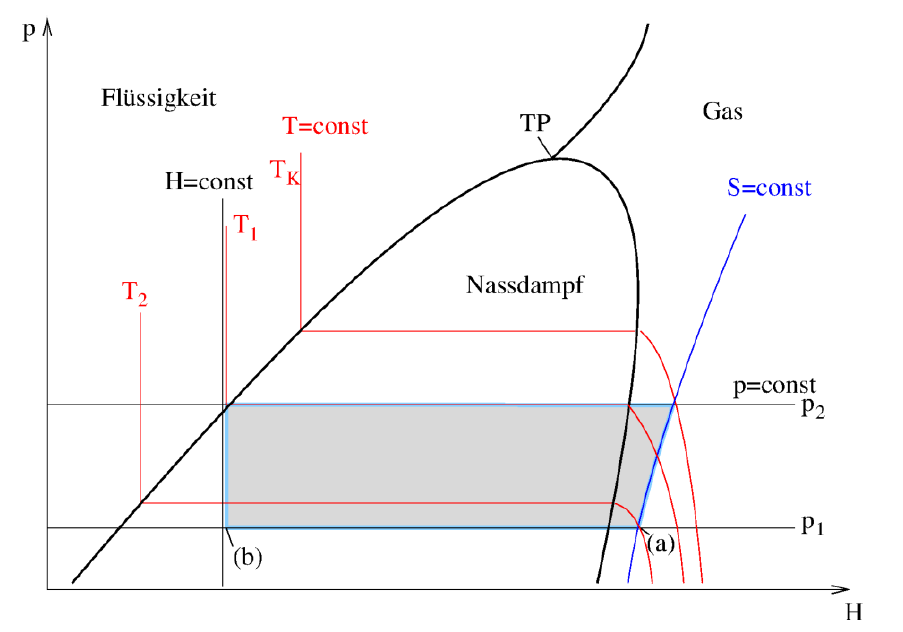
\includegraphics[width =0.8\textwidth]{./figures/ph_diagramm_grundlagen.PNG}
	\end{center}
	\caption[p-H Diagramm des Kreisprozesses]{p-H Diagramm des Kreisprozesses
		\cite{hohenau_warmepumpe_2014}
	}\label{fig:ph_diagramm_grundlagen}
\end{figure}

Der Kältekreislauf besteht aus vier Hauptstufen \cite{hohenau_warmepumpe_2014}:

\begin{enumerate}
	\item Isentrope Verdichtung: Das Kältemittel wird durch einen Kompressor komprimiert,
	      wodurch Druck und Temperatur erhöht werden. Diese Stufe wird durch eine Linie
	      dargestellt, die von niedrigem Druck und niedriger Enthalpie zu hohem Druck und
	      hoher Enthalpie isentrop verläuft.
	\item Isobare Kondensation: Das unter hohem Druck stehende und auf hohe Temperatur
	      gebrachte Kältemittel wird in einem Verflüssiger abgekühlt, wo es Wärme abgibt
	      und zu einer Flüssigkeit kondensiert. Diese Stufe wird wird durch eine
	      horizontale Linie dargestellt, die von hoher Enthalpie zu niedriger Enthalpie
	      verläuft, während der Druck konstant bleibt.
	\item Isenthalpe Drosselung: Das flüssige Kältemittel wird durch ein Expansionsventil
	      geleitet, wo sein Druck verringert wird, wodurch es zu einem Gas mit niedrigem
	      Druck verdampft. Diese Stufe wird durch eine Linie dargestellt, die bei
	      konstanter Enthalpie verläuft, während der Druck abnimmt.
	\item Isobare Verdampfung: Das Niederdruck-Kältemittel absorbiert Wärme beim
	      Verdampfer aus der Umgebung, die es kühlen soll, und kehrt zum Kompressor
	      zurück, um den Kreislauf erneut zu starten. Diese Phase wird durch eine Linie
	      dargestellt, die von niedriger Enthalpie zu hoher Enthalpie verläuft, während
	      der Druck konstant bleibt.
\end{enumerate}

\subsection{Solarzelle}
Eine Solarzelle, die auch als photovoltaische Zelle bezeichnet wird, wandelt
Sonnenlicht durch den Photoeffekt in elektrische Energie um. Der Photoeffekt
ist das Phänomen, bei dem ein Material Photonen (Lichtteilchen) absorbiert und
freie Elektronen und Löcher erzeugt, die zur Erzeugung von elektrischem Strom
genutzt werden können.

Die Grundstruktur einer Solarzelle besteht aus einer dünnen Halbleiterschicht,
die in der Regel aus Silizium besteht. Diese Halbleiterschicht befindet sich
zwischen zwei Metallkontakten, von denen einer auf der Ober- und einer auf der
Unterseite liegt. Wenn Sonnenlicht auf die Halbleiterschicht fällt, werden die
Photonen des Sonnenlichts von dem Halbleitermaterial absorbiert. Dies führt
dazu, dass einige der Elektronen im Material angeregt werden und auf ein
höheres Energieniveau springen, wobei ein \dq Loch\dq \ im Material
zurückbleibt, wo das Elektron vorher war.

Die angeregten Elektronen und die durch die absorbierten Photonen entstandenen
Löcher werden dann durch das elektrische Feld getrennt, das durch den Übergang
zwischen den beiden Schichten des Halbleiters entsteht. Dieses elektrische Feld
wird durch Dotierung des Halbleiters mit Verunreinigungen erzeugt, um einen
p-n-Übergang zu schaffen. Die p-Typ-Halbleiterschicht hat einen Überschuss an
positiv geladenen Löchern, während die n-Typ-Schicht einen Überschuss an
negativ geladenen Elektronen hat.

Die angeregten Elektronen werden in Richtung der n-Typ-Schicht gezogen, während
die Löcher in Richtung der p-Typ-Schicht gezogen werden. Durch diese
Ladungstrennung entsteht eine Spannungsdifferenz über der Halbleiterschicht,
die zur Erzeugung elektrischer Energie genutzt werden kann. Die schematische
Funktionsweise der Solarzelle ist in folgender
\autoref{fig:solarzelle_grundlagen} ersichtlich.

\begin{figure}[H]
	\begin{center}
		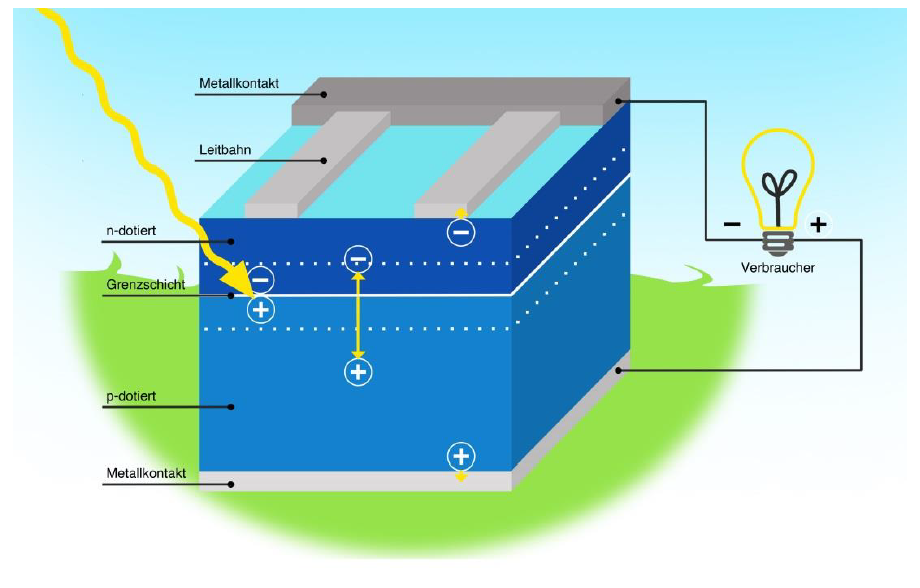
\includegraphics[width =0.8\textwidth]{./figures/solarzelle_grundlagen.PNG}
	\end{center}
	\caption[Schematische Funktionsweise der Solarzelle]{Schematische Funktionsweise der
		Solarzelle~\cite{knoll_solarzelle_nodate}
	}\label{fig:solarzelle_grundlagen}
\end{figure}

Die Shockley-Gleichung beschreibt die Beziehung zwischen dem Stromdurchsatz
einer Diode und der an ihr anliegenden Spannung. Da eine Solarzelle nichts
anderes als eine Diode ist, gilt dieses Gesetz auch in diesem Fall. Die
Shockley-Gleichung kann verwendet werden, um die Diodenkennlinie einer
Solarzelle anzupassen und wichtige Parameter wie den Fotostrom, den
Sättigungsrückstrom und den Idealitätsfaktor zu ermitteln. Diese Informationen
sind nützlich, um die Leistung einer Solarzelle zu bewerten und ihr Design für
eine maximale Effizienz zu optimieren.

Aus der Shockley-Gleichung geht unter Berücksichtigung der parasitären
Widerstände die \autoref{eq:I_eindiodenmodell} für den gemessen Strom $I$
hervor. Berücksichtigt man, dass in der Solarzelle Dotierungsschwankungen
vorherschen, bezeichnet das Zweidiodenmodell aus
\autoref{eq:I_zweidiodenmodell} eher das tatsächliche Verhalten.

\begin{equation}
	I=I_{S 1}\left(e^{\frac{e\left(U-I R_s\right)}{f_1 k_B T}}-1\right)-I_{p h}+\frac{\left(U-I R_s\right)}{R_p}
	\label{eq:I_eindiodenmodell}
\end{equation}

\begin{equation}
	I=I_{S 1}\left(e^{\frac{e\left(U-I R_s\right)}{f_1 k_B T}}-1\right)+I_{S 2}\left(e^{\frac{e\left(U-I R_s\right)}{f_2 k_B T}}-1\right)-I_{p h}+\frac{\left(U-I R_s\right)}{R_p}
	\label{eq:I_zweidiodenmodell}
\end{equation}

$I_{S 1}$ bzw. $I_{S 2}$ bezeichnet dabei den Sättigungsstrom,
$U$ die gemessene Spannung,
$R_{s}$ den Serienwiderstand,
$R_p$ den Parallelwiderstand,
$k_B$ die Boltzmann-Konstante,
$e$ die Elementarladung,
$T$ die absolute Temperatur,
$I_{ph}$ den Betrag des Photostroms und
$f_1$ bzw $f_2$ die Diodenfaktoren zur Anpassung.

Die Diodenkennlinie einer Solarzelle kann zur Bewertung und Charakterisierung
der Leistung der Zelle verwendet werden. Durch die Analyse der Diodenkennlinie
können die folgenden Schlüsselparameter der Solarzelle nach den folgenden
Formeln bestimmt werden:

\begin{enumerate}
	\item Leerlaufspannung ($U_L$): Dies ist die Spannung, bei der die Solarzelle keinen
	      Strom erzeugt, und entspricht der maximalen Ausgangsspannung der Zelle. Die
	      Leerlaufspannung wird durch die Beleuchtungsstärke und die intrinsischen
	      Eigenschaften der Zelle bestimmt.
	\item Kurzschlussstrom ($I_k$): Dies ist der Strom, der von der Solarzelle erzeugt
	      wird, wenn die Spannung über der Zelle gleich Null ist, und entspricht der
	      maximalen Stromabgabe der Zelle. Der Kurzschlussstrom wird durch die
	      Beleuchtungsstärke und die physikalischen Eigenschaften der Zelle bestimmt.
	\item Füllfaktor ($FF$): Er ist ein Maß für den Wirkungsgrad der Solarzelle und wird
	      durch das Verhältnis zwischen der maximalen Ausgangsleistung der Zelle und dem
	      Produkt aus Leerlaufspannung und Kurzschlussstrom bestimmt. Der Füllfaktor wird
	      von den physikalischen Eigenschaften der Zelle, wie der Rekombinationsrate und
	      dem Serien- und Nebenschlusswiderstand, beeinflusst.
	\item Maximaler Leistungspunkt (MPP): Dies ist der Punkt auf der Diodenkennlinie, an
	      dem die Solarzelle die maximale Leistung abgibt. Der Punkt maximaler Leistung
	      wird von der Beleuchtungsstärke und den physikalischen Eigenschaften der Zelle
	      beeinflusst.
\end{enumerate}

\begin{equation}
	FF=\frac{I_{\text {max }} U_{\max }}{I_K U_L}
	\label{eq:I_fuellfaktor}
\end{equation}

\begin{equation}
	P_\text{MPP} =I_{\max } U_{\max }
	\label{eq:leistung_max}
\end{equation}

\begin{equation}
	\eta=\frac{P_{\text {max }}}{P_{\text {Licht }}}
	\label{eq:wirkungsgrad_solar}
\end{equation}

\begin{equation}
	P_{\text {Licht }}=A \cdot I_{\text {Licht}} \quad I_{\text {Licht }}=\frac{P_{\text {mess }}}{A_{\text {mess }}} \\
	\label{eq:leistung_solar}
\end{equation}

$U_{\max}$ bezeichnet dabei die Spannung beim Punkt maximaler Leistung,
$I_{\max}$ die Stromstärke beim Punkt maximaler Leistung,
$\eta$ den entsprechenden Wirkungsgrad,
$P_{\text {Licht }}$ die gemessene Leistung am Strahlungsmessgerät,
$A$ die aktive Fläche der Solarzelle,
$I_{\text {Licht }}$ die Lichtintensität der Lampe,
$P_{\text {mess }} $ die gemessene Leistung am Strahlungsmessgerät und
$A_{\text {mess }} $ die Fläche des Leistungsmessgeräts.

Durch die Auswertung und Analyse dieser Schlüsselparameter kann die
Diodenkennlinie wertvolle Erkenntnisse über die Leistung einer Solarzelle
liefern. Diese Informationen können dazu genutzt werden, das Design der
Solarzelle zu optimieren und ihren Wirkungsgrad und ihre Leistung zu
verbessern~\cite{knoll_solarzelle_nodate}.

\section{Versuchsanordnung}\label{sec:versuchsanordnung}

\subsection{Wärmepumpe}

Der reale Versuchsaufbau,\autoref{fig:warmepumpe}, sowie eine schematische
Skizze dessen, \autoref{fig:skizze_warmepumpe}, sind im folgenden sichtbar.

\begin{figure}[H]
	\begin{center}
		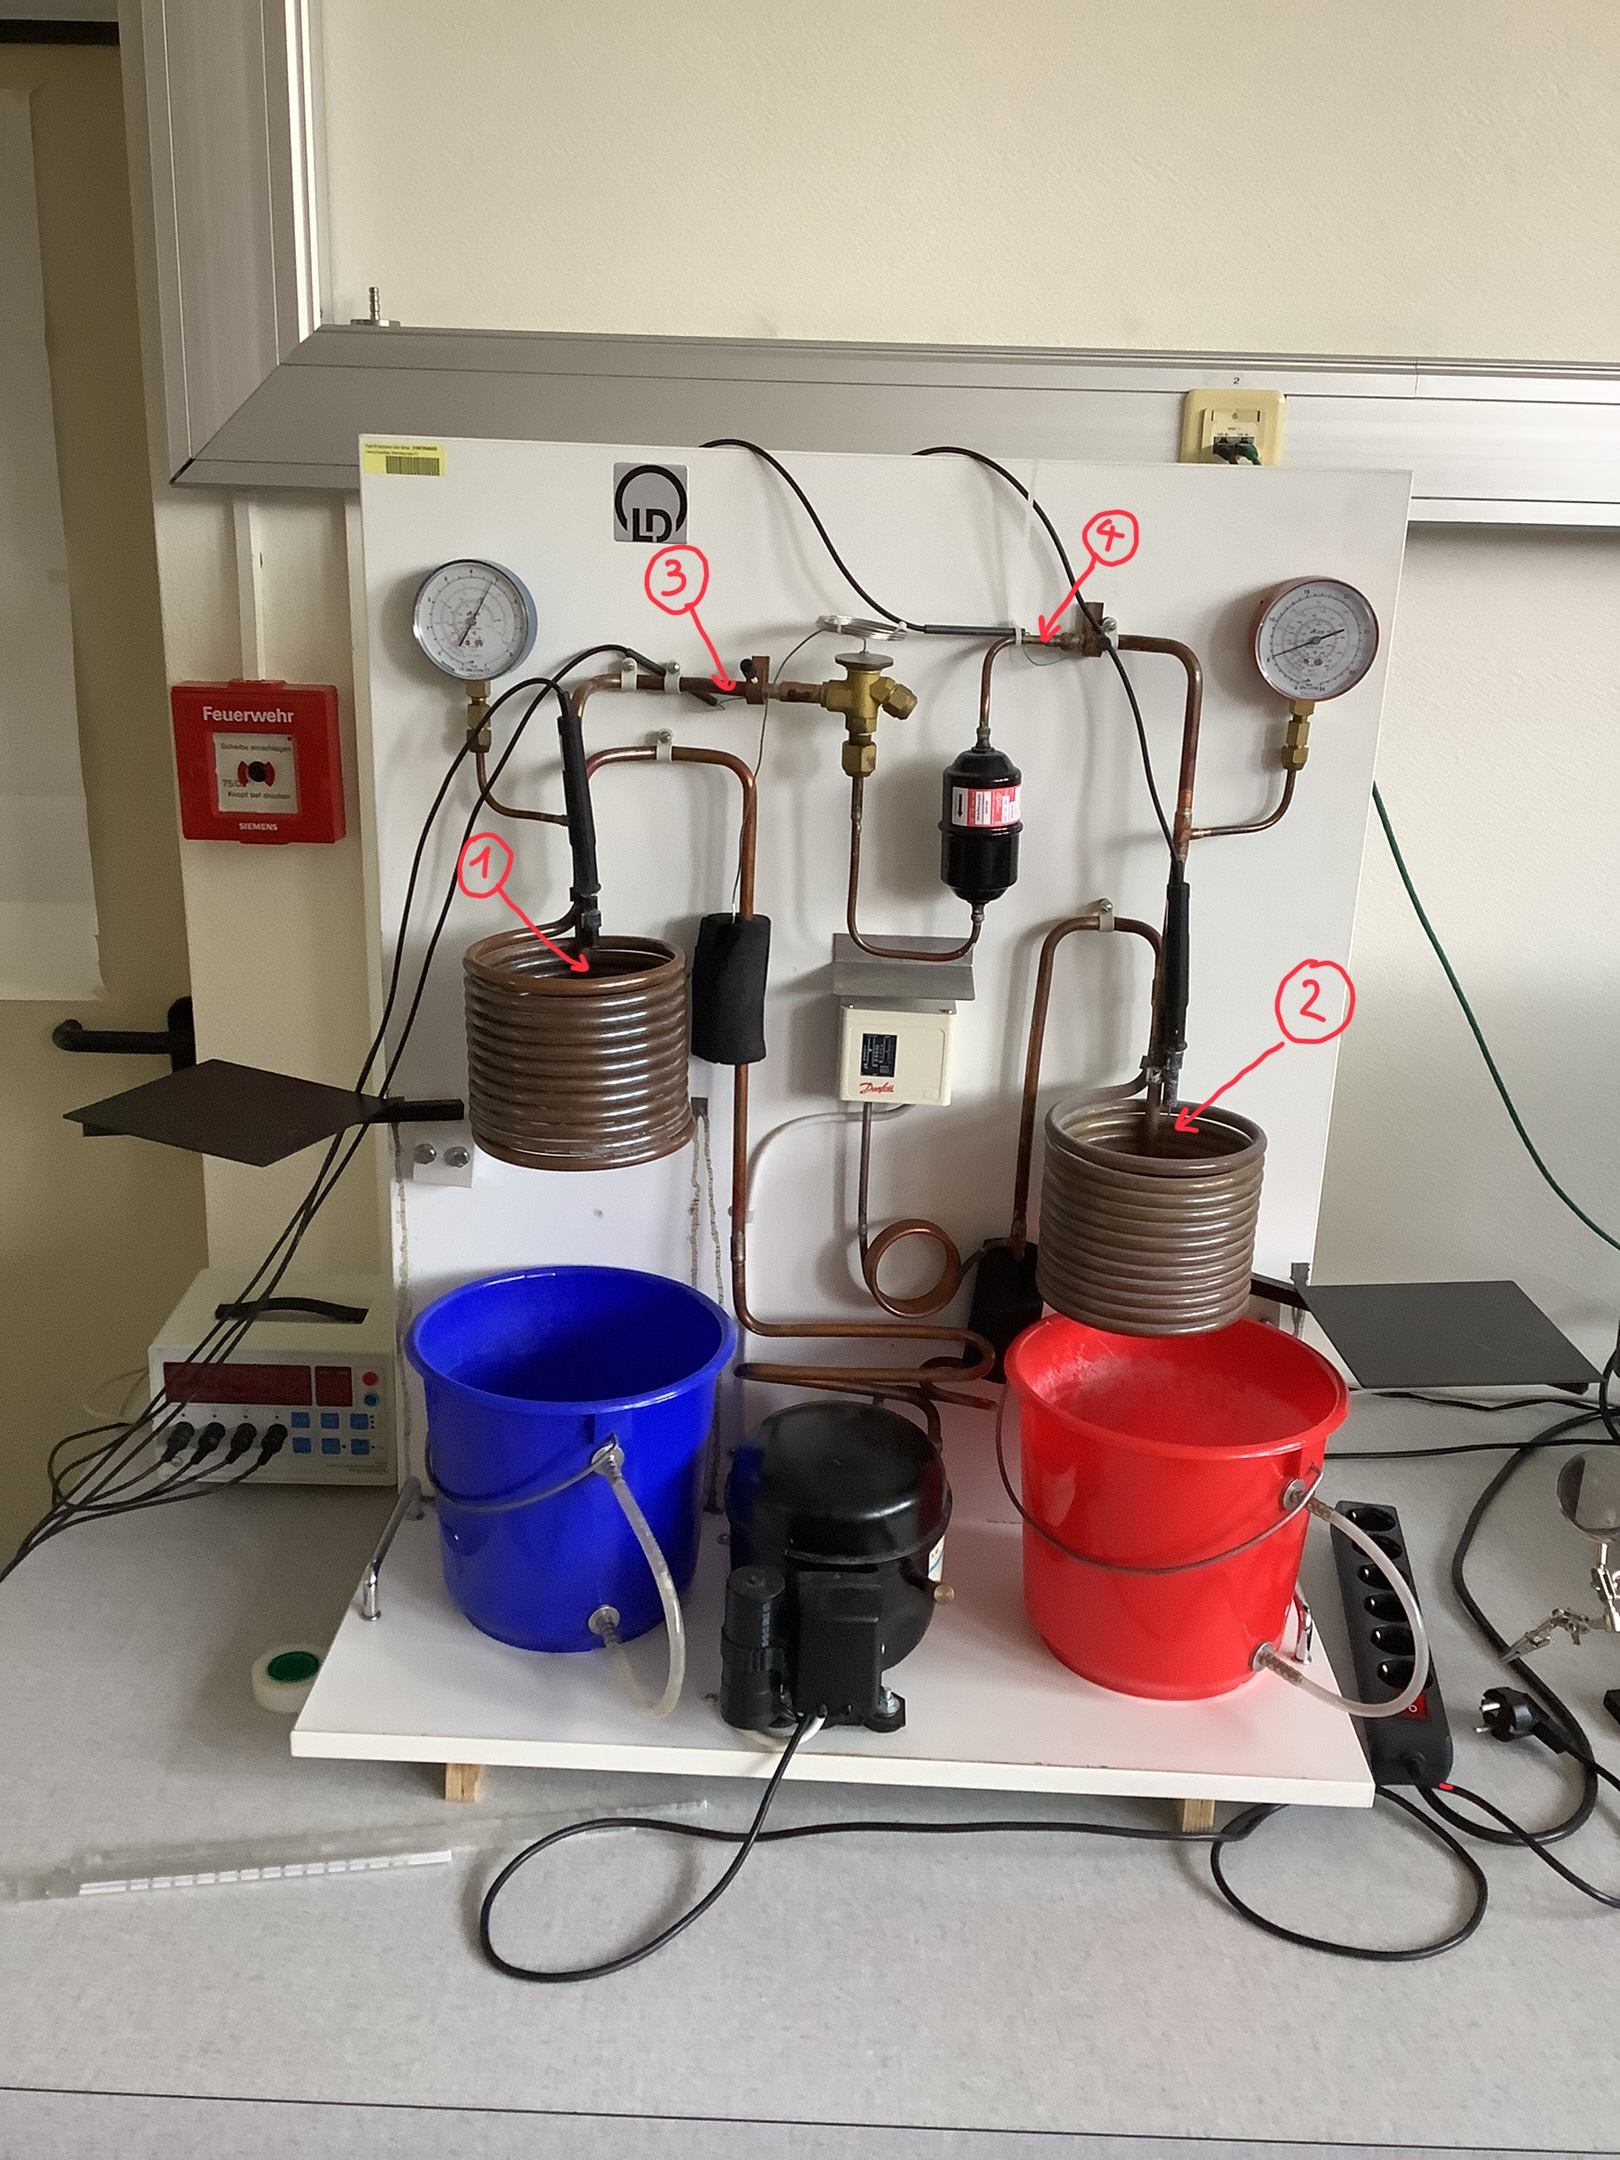
\includegraphics[width =0.5\textwidth]{./figures/warmepumpe_anschlusse.png}
	\end{center}
	\caption[Versuchsaufbau der Wärmepumpe]{Versuchsaufbau der Wärmepumpe, am Bild markiert
		sind die Kanäle, mit denen die entsprechenden Temperatursensoren verbunden sind
	}\label{fig:warmepumpe}
\end{figure}

\begin{figure}[H]
	\begin{center}
		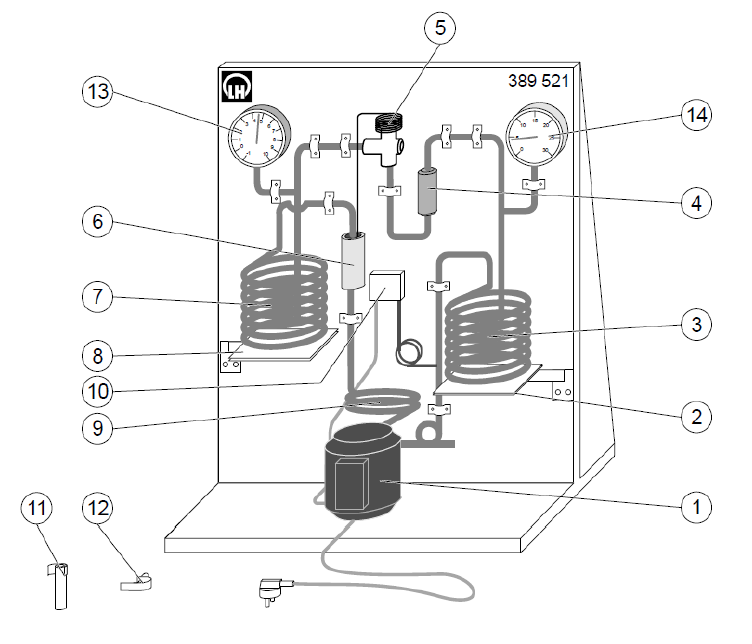
\includegraphics[width =0.5\textwidth]{./figures/warmepumpe_skizze.PNG}
	\end{center}
	\caption[Skizze des Versuchsaufbaus der Wärmepumpe]{Skizze des Versuchsaufbaus der
		Wärmepumpe~\cite[text]{hohenau_warmepumpe_2014}.                          \\
		1 \dots Kompressor 230 V; 50/60 Hz. Leistungsaufnahme ca. 130 W bei 50 Hz \\
		2 \dots ausschwenkbare Stellfläche für rot-markierten Warmwasserbehälter  \\
		3 \dots Verflüssiger                                                      \\
		4 \dots Sammler/Reiniger                                                  \\
		5 \dots Expansionsventil                                                  \\
		6 \dots Temperaturfühler des Expansionsventils                            \\
		7 \dots Verdampfer                                                        \\
		8 \dots ausschwenkbare Stellfläche Kaltwasserbehälter                     \\
		9 \dots Rohrwindungen als elastische Verbindung zwischen Kompressor und
		Wärmetauscher                                                             \\
		10 \dots Druckwächter                                                     \\
		11 \dots Kunststoffhalter (2x) für Thermometer und Temperaturfühler, zum
		Anklemmen an Kupferrohre                                                  \\
		12 \dots Kupfer-Meßschuh (2x) zum Einstecken von Temperaturfühlern für
		Temperaturmessungen an den Kupferrohren des Kältemittelkreislaufs         \\
		13 \dots Manometer für die Niederdruckseite; innere Skala für Druckmessung von
		-1...+10 bar, äußerste Skala mit zugehöriger Taupunkttemperatur für R134a von
		-60 °C bis +40 °C                                                         \\
		14 \dots Manometer für die Hochdruckseite; innere Skala: Druck von -1...+30
		bar, äußerste Skala mit zugehöriger Taupunkttemperatur für R 134a von -60 °C
		bis + 85°C.
	}\label{fig:skizze_warmepumpe}
\end{figure}

Die Temperatursensoren werden mit dem Temperaturmessgerät, wie in
\autoref{fig:warmepumpe} sichtbar, verbunden. Das Temperaturmessgerät wird über
die USB-Schnittstelle mit den Rechner verbunden, um eine Auswertung mit der
Software Cassy Lab2 zu ermöglichen.

Weil der Temperatursensor im kälteren Behälter laufend zur Spule gerutscht ist
und dies die Messung verfälschen würde, wurde er mit einem Stück Lötzinn gegen
Verrutschen gesichert, wie in \autoref{fig:lotzinn} sichtbar.

\begin{figure}[H]
	\begin{center}
		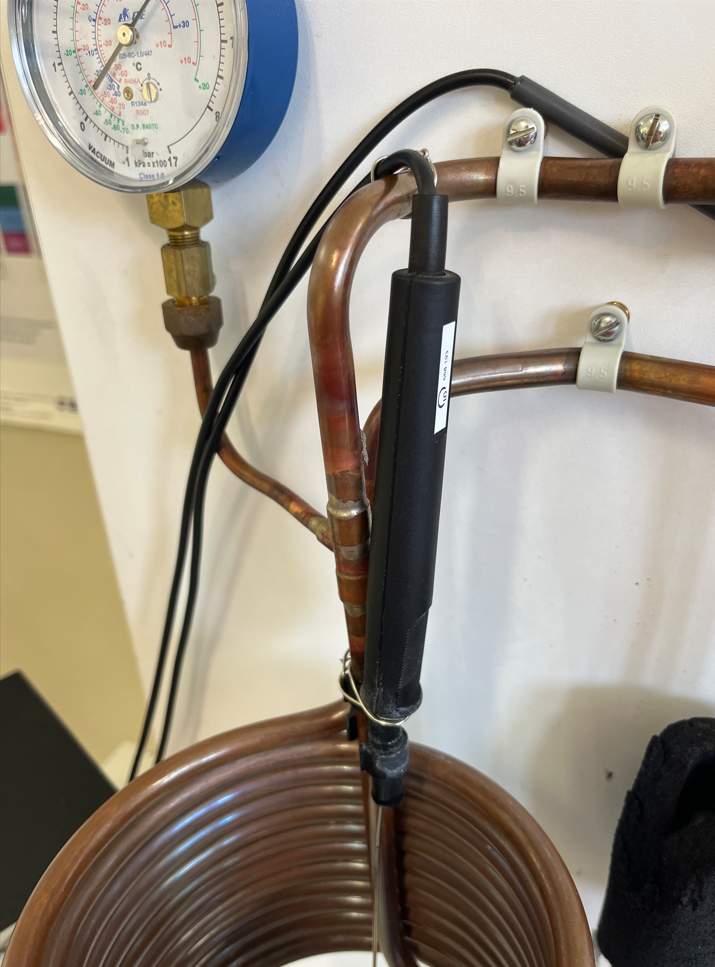
\includegraphics[width =0.5\textwidth]{./figures/lotzinn.png}
	\end{center}
	\caption{Sicherung gegen Verrutschen des Temperatursensors
	}\label{fig:lotzinn}
\end{figure}

\subsection{Kennlinien und Kenndaten von Solarzellen bei Bestrahlung}

Um die Kennlinie der Solarzelle zu bestimmen wird diese, der jeweiligen
Schaltung entsprechend, an einen verstellbaren Widerstand geschlossen. Damit
Messwerte generiert werden können, werden auch ein Amperemeter, sowie ein
Voltmeter nach dem Schaltplan in \autoref{fig:schaltplan} in die Schaltung
integriert. Bei den Messgeräten muss darauf geachtet werden, einen geeigneten
Messbereich zu wählen.

\begin{figure}[H]
	\begin{center}
		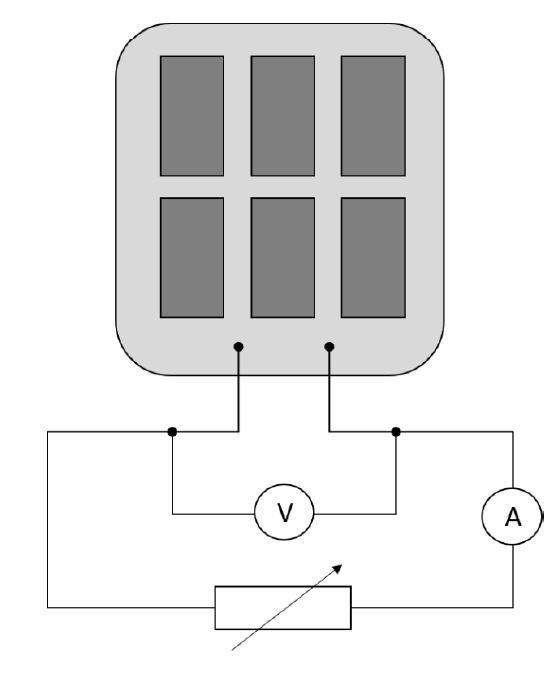
\includegraphics[width =0.5\textwidth]{./figures/schaltplan.PNG}
	\end{center}
	\caption[Schaltplan der Solarzelle]{Schaltplan der
		Solarzelle~\cite{knoll_solarzelle_nodate} \\
		A \dots Amperemeter                       \\
		V \dots Voltmeter
	}\label{fig:schaltplan}
\end{figure}

Die folgenden Abbildungen zeigen die Serienschaltung,
\autoref{fig:Serienschaltung}, sowie die Parallelschaltung,
\autoref{fig:Parallelschaltung}. Um eine bessere Übersicht zu gewährleisten,
wird bei den verwendeten Kabeln auf die Farbe geachtet.

\begin{figure}[H]
	\centering
	\captionbox[Serienschaltung der beiden Solarzellen]{Serienschaltung der beiden Solarzellen\\
		1 \dots Solarzellenmodule\\
		2 \dots Lampe\\
		3 \dots regelbarer Widerstand\\
		4 \dots Voltmeter\\
		5 \dots Amperemeter\\
		6 \dots entsprechende Verkabelung für
		Serienschaltung\label{fig:Serienschaltung}}{
		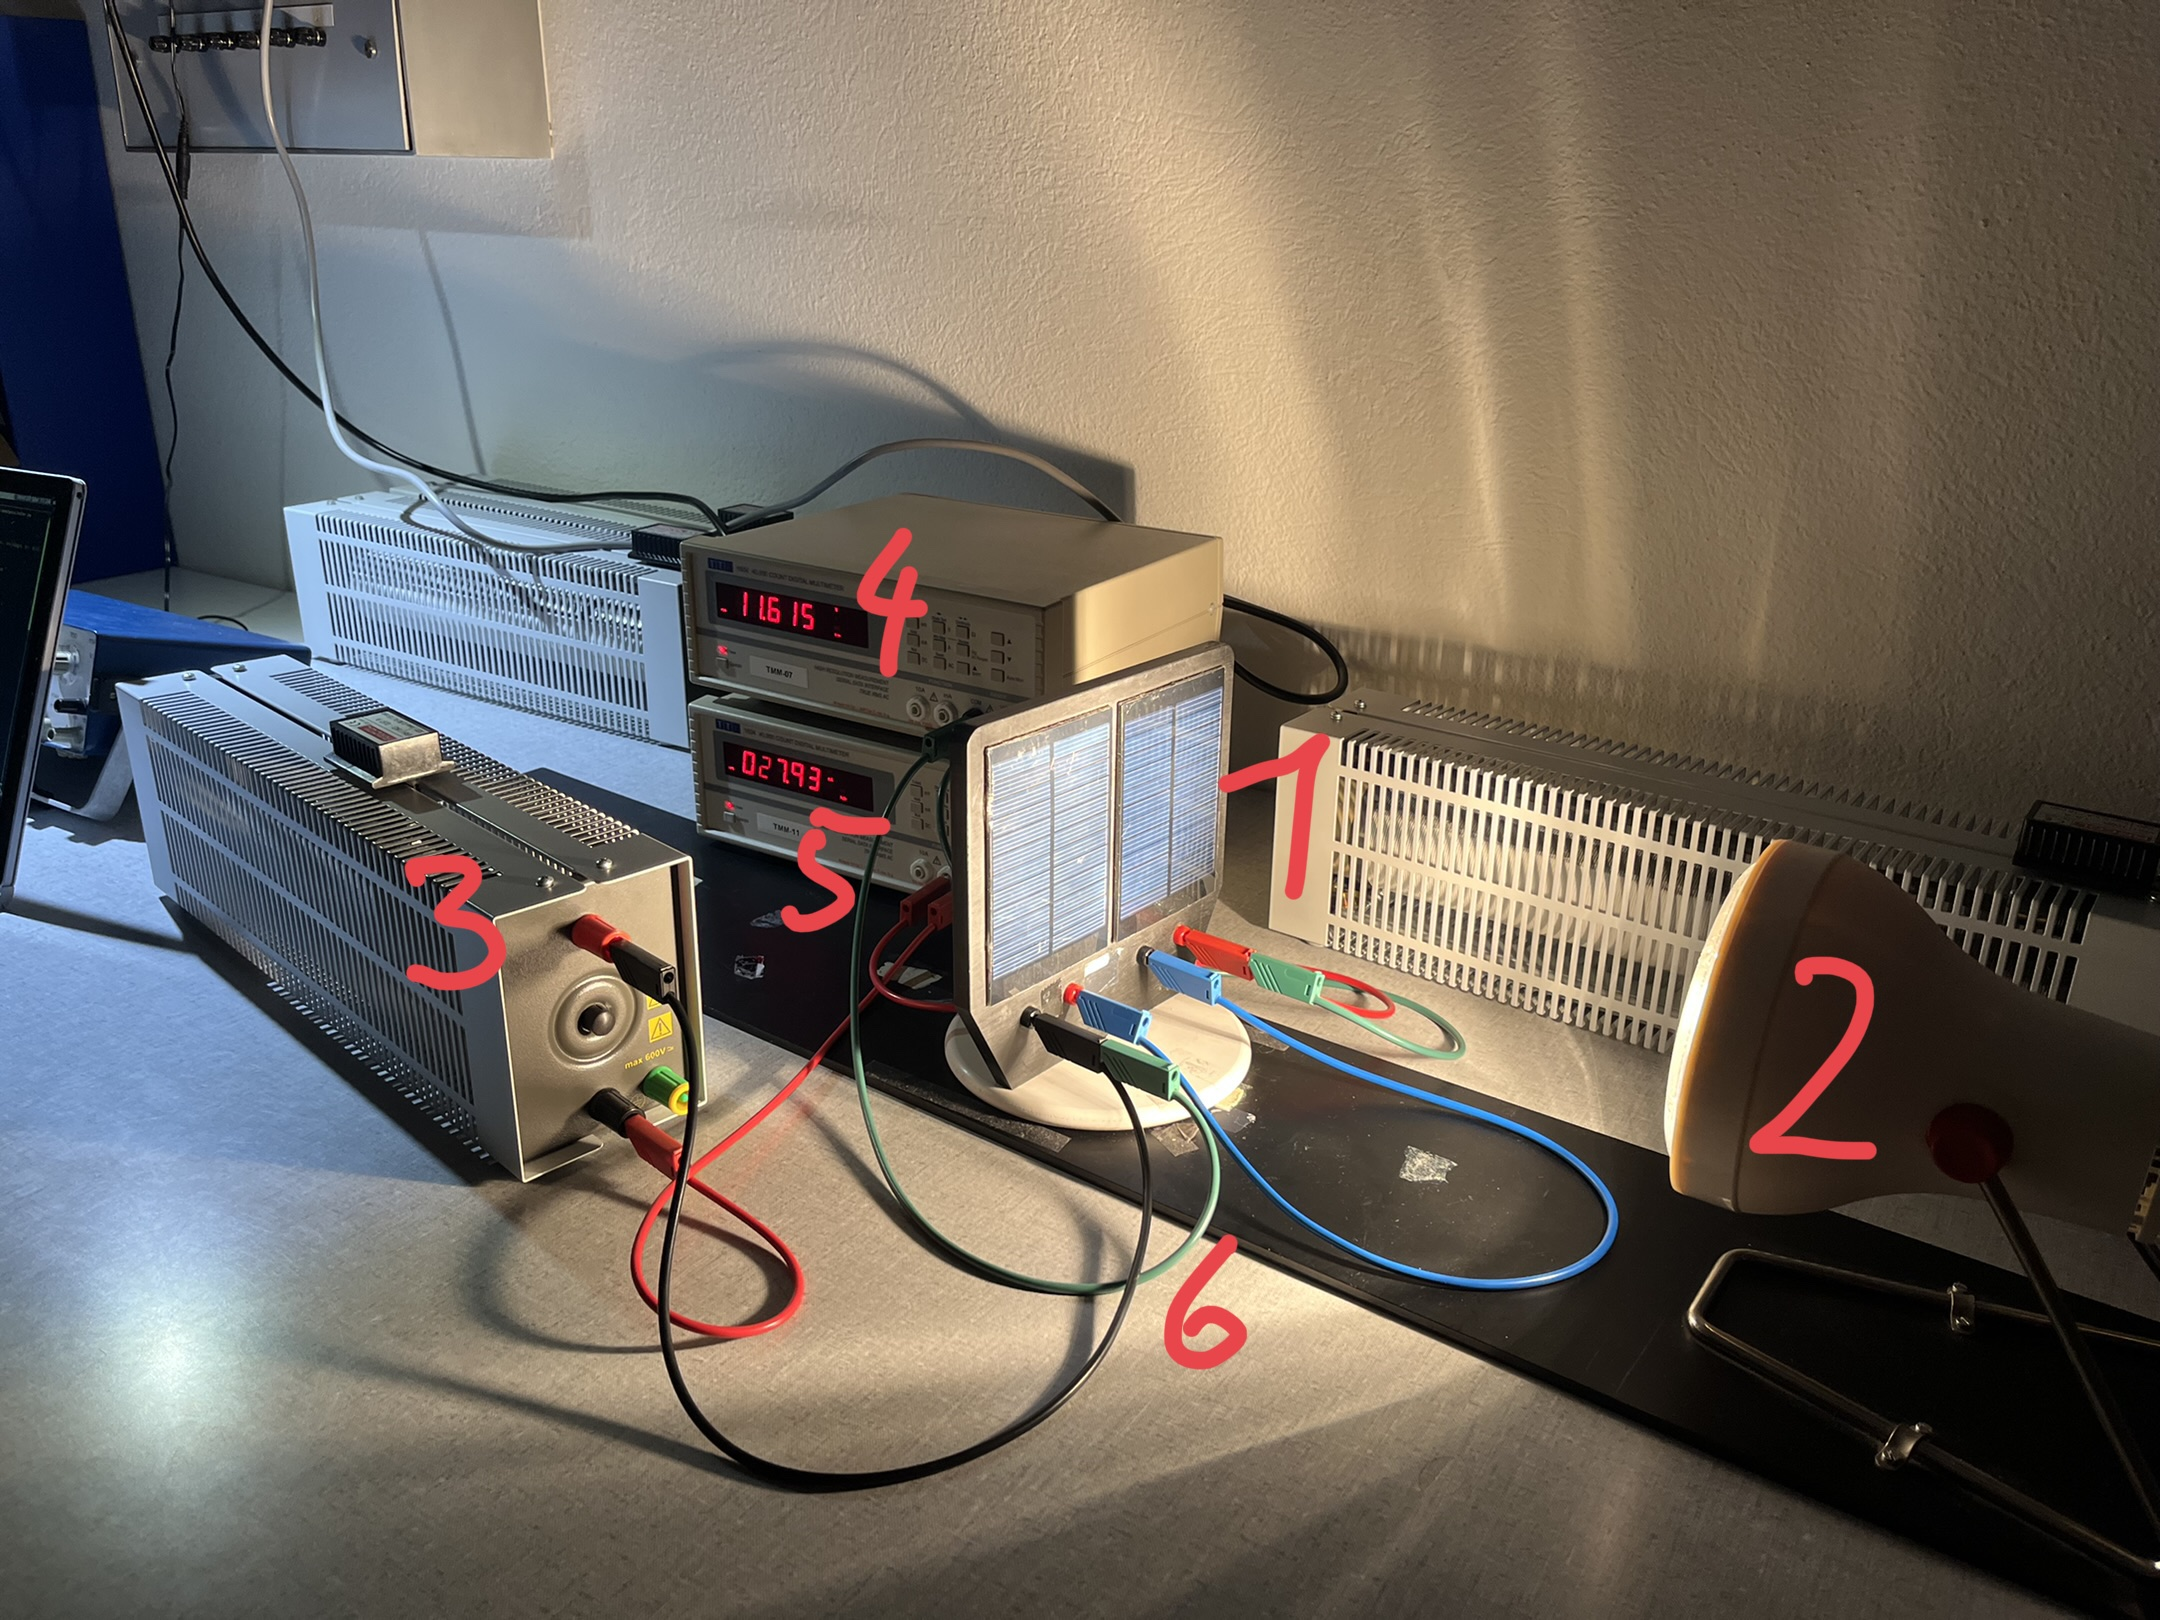
\includegraphics[width=.45\textwidth]{./figures/serienschaltung.jpg} } \hfill
	\captionbox[Parallelschaltung der beiden Solarzellen]{Parallelschaltung der
		beiden Solarzellen \\
		1 \dots Solarzellenmodule\\
		2 \dots Lampe\\
		3 \dots regelbarer Widerstand\\
		4 \dots Voltmeter\\
		5 \dots Amperemeter\\
		6 \dots entsprechende Verkabelung für
		Parallelschaltung\label{fig:Parallelschaltung}}{
		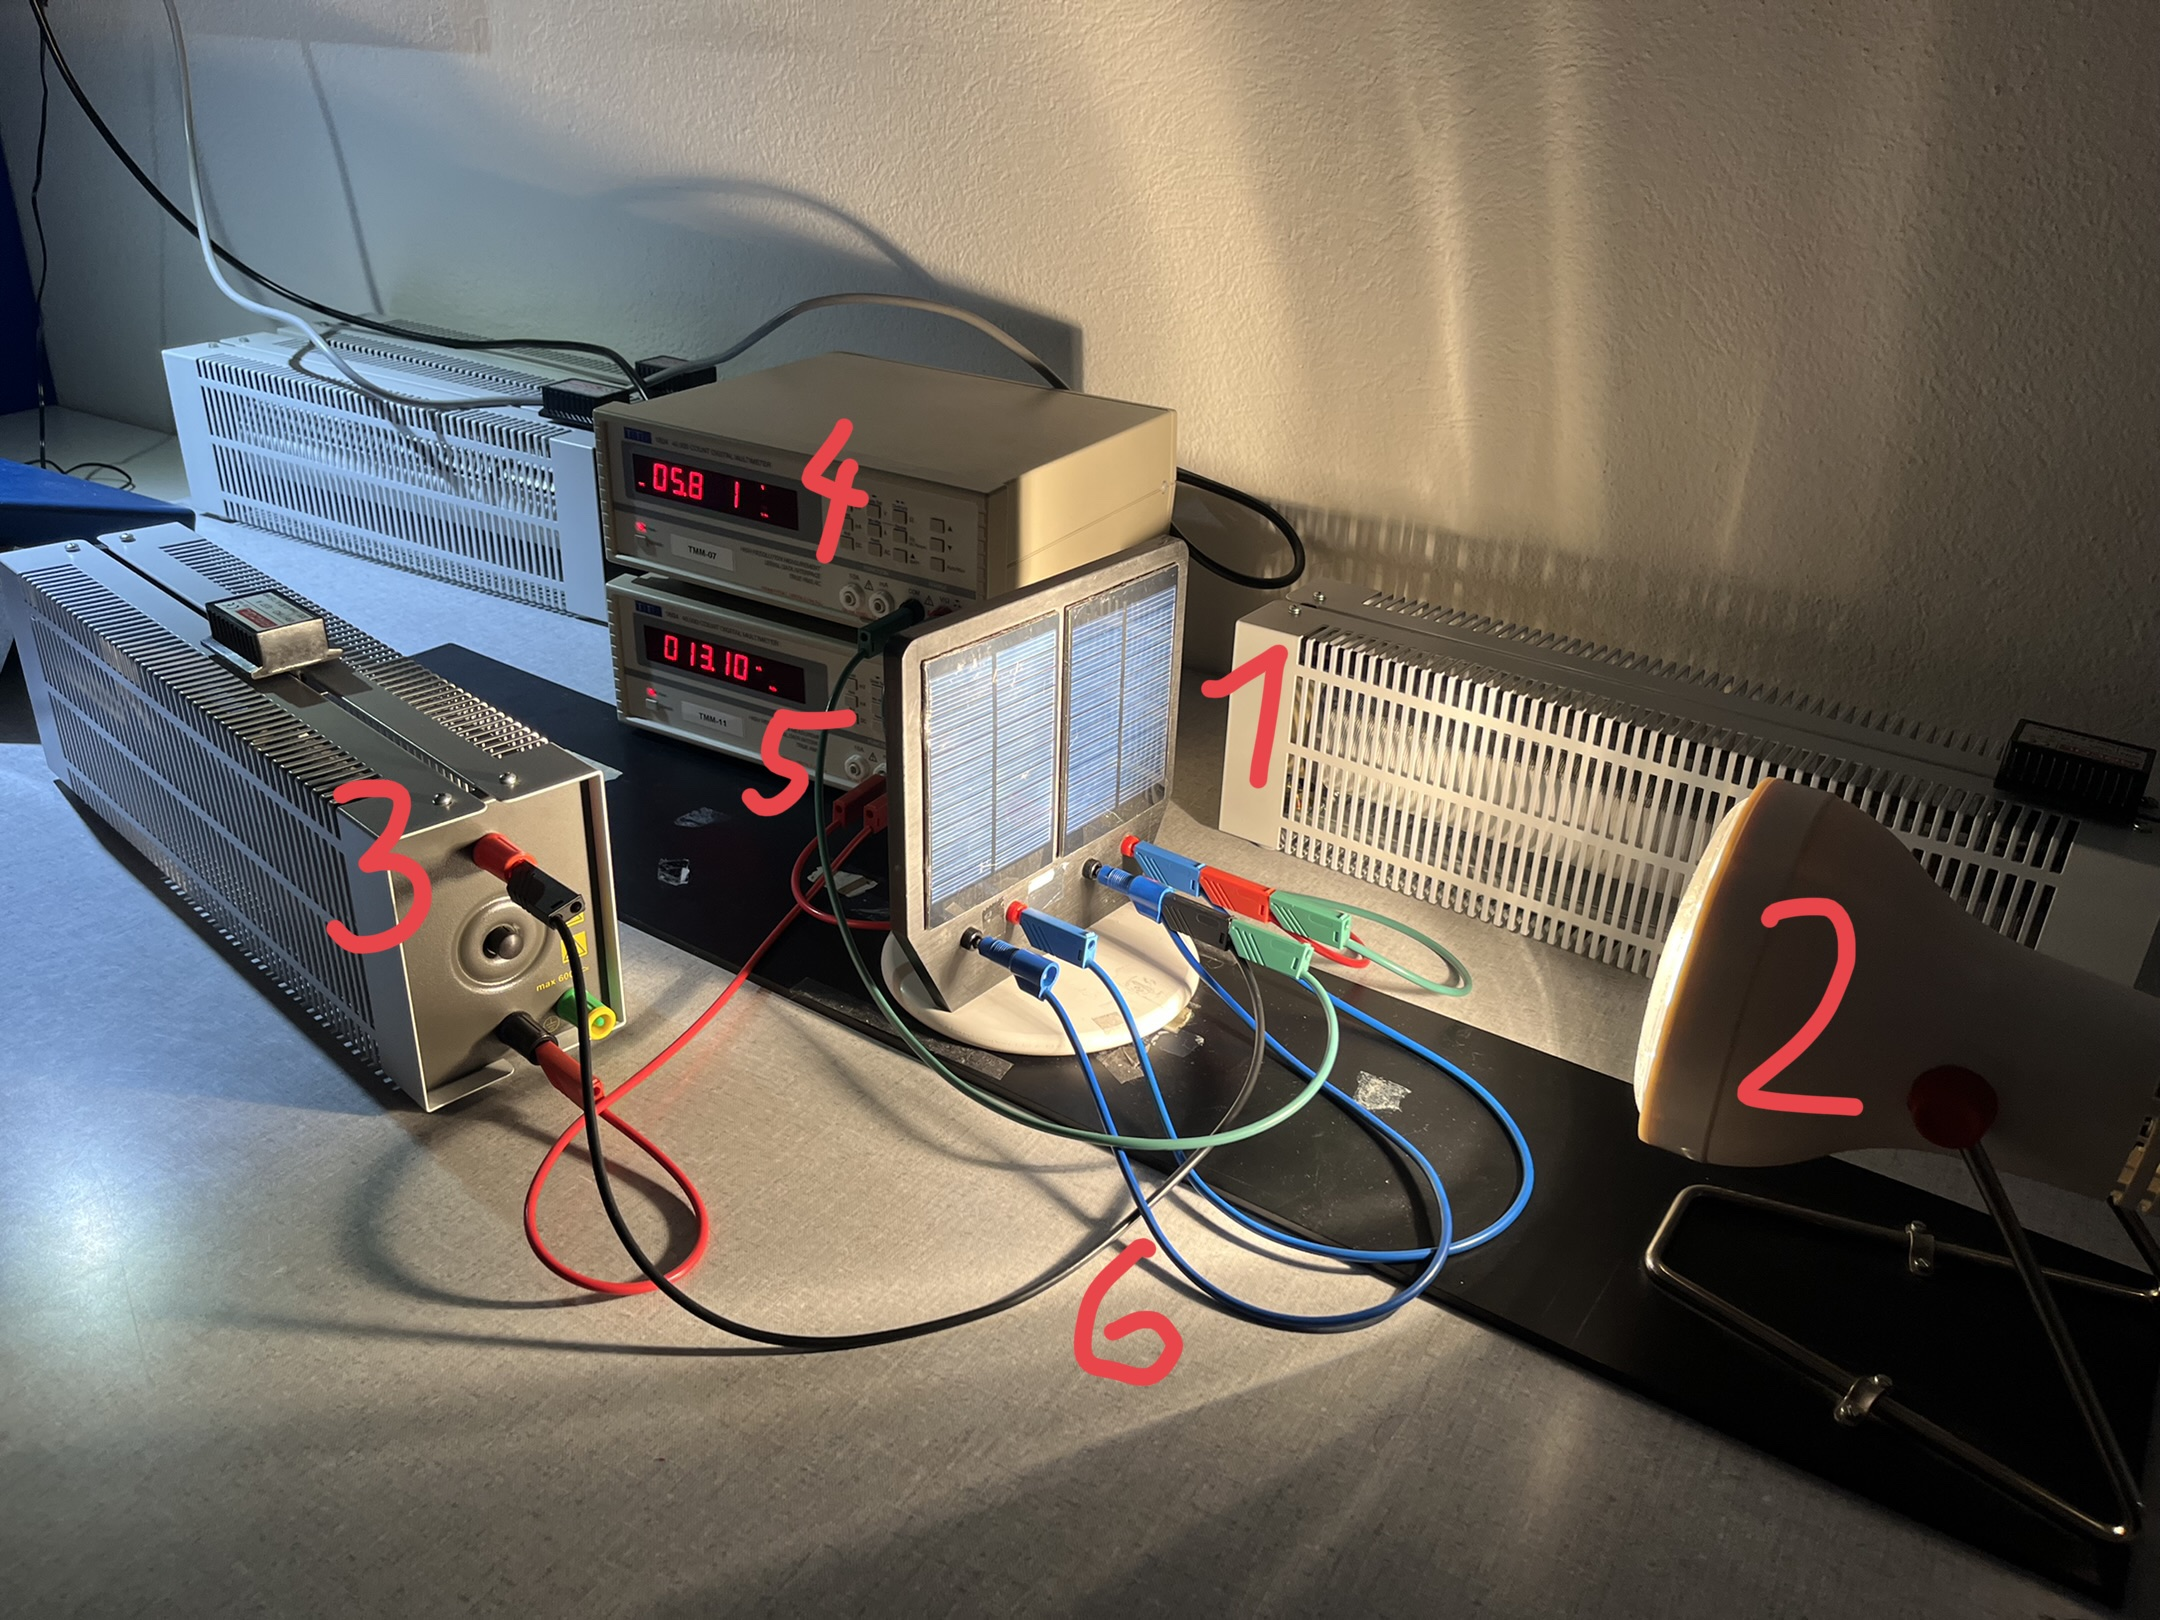
\includegraphics[width=0.45\textwidth]{./figures/parallelschaltung.jpg} }
\end{figure}

\subsubsection{Serienschaltung der beiden Solarzellen, wobei eine Solarzelle partiell abgeschattet wird}

Um die partielle Abschattung einer Solarzelle zu simulieren, wird ein Stück
Papier über einen Teil der ersten Solarzelle gelegt. Um sicherzustellen, dass
das Papier sich nicht von der Solarzelle löst, wird dieses mit Klebeband gegen
verrutschen gesichert. Dabei wird darauf geachtet, dass das Klebeband nur am
Plastikrahmen festgeklebt wird, damit keine Kleberückstände auf der Solarzelle
zurückbleiben. Die Abdunkelung ist in \autoref{fig:abgedeckt} sichtbar.

\begin{figure}[H]
	\begin{center}
		\includegraphics[width =0.5\textwidth]{./figures/abgedeckt.png}
	\end{center}
	\caption{Partielle Beschattung einer Solarzelle
	}\label{fig:abgedeckt}
\end{figure}

\subsection{Diodenparameter und Wirkungsgrad einer Solarzelle}

Um den Diodenparameter, sowie den Wirkungsgrad der Solarzelle zu bestimmen,
wird diese auf den entsprechenden Kupferbock zur Kühlung gelegt. Der Sensor
wird neben die Solarzelle positioniert und mit einem Block unterlegt, damit
sich der Sensor auf der gleichen Höhe, wie die Solarzelle befindet.

Um die Diodenkennlinie aufzuzeichnen wird das Keithley 2450 also Sourcemeter
verwendet. Dieses wird über eine USB Schnittstelle mit dem Rechner verbunden.
Um den Fehler bei der Spannungsmessung möglichst gering zu halten, wird die
Solarzelle mit 4 Kabeln mit dem Sourcemeter verbunden, wobei 2 der
Sense-Leitung entsprechen.

Weil der Sonnensimulator leider kaputt war wurden als Lichtquelle eine
höhenverstellbare Halogenlampe, sowie eine LED Beleuchtung verwendet. Aus
Neugierde wurde der Versuch für 2 verschiedene Abstände der Halogenlampe und
einmal für die LED Beleuchtung durchgeführt. Bei der Position der Lampe muss
darauf geachtet werden, dass der Abstand zwischen der Lampe und der Solarzelle
oder dem Sensor konstant gehalten werden soll. Auch wird sichergestellt, dass
die Lichtquelle immer ober dem Objekt zentriert wird. Um Störlicht von der
Umgebung zu vermeiden, wird der Versuch bei ausgeschalteter Raumbeleuchtung und
geschlossenen Türen durchgeführt, um sicherzustellen, dass nur das gewünschte
Licht von der, zu untersuchenden Lichtquelle auf den Sensor oder die Solarzelle
trifft.

\section{Geräteliste}\label{sec:geraeteliste}

Für die Wärmepumpe werden die in \autoref{tab:gerate_warme} aufgelisteten
Geräte verwendet.

\begin{table}[H]
	\caption{Verwendete Geräte für die Wärmepumpe
	}
	\begin{tblr}{cells={font=\footnotesize},colspec={lllll}}
		\textbf{Gerätetyp}  & \textbf{Hersteller} & \textbf{Typ}   & \textbf{Inventar-Nr} & \textbf{Anmerkung} \\
		Wärmepumpe          & LD                  &                &                      &                    \\
		Kompressor          & Danfoss             & TL3G           & AA6HA100             & \SI{118(2)}{\watt} \\
		Druckwächter        & Danfoss             &                &                      &                    \\
		Sammler             & UL                  & 16H5           & 023Z4566             &                    \\
		Temperaturfühler    &                     & Ni Cr-Ni       &                      & 4x                 \\
		Barometer           & ITE                 & 823-BC-1.0/447 &                      & für warm           \\
		Barometer           & ITE                 & 825-BC-1.0/447 &                      & für kalt           \\
		Temperatormessgerät & LD                  & 666209         & TOP0000252           & mit 4 Anschlüssen  \\
		Computersoftware    & Cassy Lab 2         &                &                      &                    \\
		Messbecher          & Vit Lab             & 2 Liter        &                      &                    \\
		Eimer               &                     &                &                      & 2x mit Schlauch    \\
		Verbindungskabel    &                     &                &                      &                    \\
		Glasstab            &                     &                &                      & zum Umrühren
	\end{tblr}\label{tab:gerate_warme}
\end{table}

Für die beiden Versuche mit den Solarzellen werden die in
\autoref{tab:gerate_solar} aufgelisteten Geräte verwendet.

\begin{table}[H]
	\caption{Verwendete Geräte für die beiden Solarzellen Versuche
	}
	\begin{tblr}{cells={font=\footnotesize},colspec={lllll}}
		\textbf{Gerätetyp}                            & \textbf{Hersteller} & \textbf{Typ} & \textbf{Inventar-Nr} & \textbf{Anmerkung}                           \\
		Solarzellenmodul                              &                     &              &                      & 2x $\SI{10.0(2)}{\cm}\cdot \SI{8.0(2)}{\cm}$ \\
		Radium-Lampe                                  &                     & PAR 38-EC    &                      &                                              \\
		Verstellbarer Widerstand                      & ARCOL               & VRH 320      & CEI 1010-1           &                                              \\
		Voltmeter                                     & TTI                 & 1604         & TMM-07               &                                              \\
		Amperemeter                                   & TTI                 & 1604         & TMM-11               &                                              \\
		Bananenstecker                                &                     &              &                      &                                              \\
		Papier                                        &                     &              &                      & zum Verdecken                                \\
		Rollmeter                                     & Schuller            & 3 m          &                      & für Distanzmessung                           \\
		Solarzellenmodul                              &                     &              &                      &                                              \\
		Leistungssensor\cite{noauthor_407a_nodate}    & Spectra Physics     & 407A         & 2775                 &                                              \\
		Leistungsmessgerät\cite{noauthor_407a_nodate} & Spectra Physics     & 407A         &
		310041630000                                  &                                                                                                          \\
		Sourcemeter\cite{noauthor_2450_nodate}        & Keithley            & 2450 S       & 300032370000         &                                              \\
		Computersoftware                              & Kickstart           &              &                      &                                              \\
		Halogenlampe                                  & Osram               & 24V 150W     & HL\% 64640           &                                              \\
		LED-lampe                                     & Hansa               & 41-5010.608  &                      &
	\end{tblr}\label{tab:gerate_solar}
\end{table}
\section{Versuchsdurchführung und Messergebnisse}\label{sec:versuchsdurchfuehrung_messergebnisse}

\subsection{Wärmepumpe}

Zunächst werden beide Kübel mit \SI{4000(40)}{\milli\liter} Wasser gefüllt. Um
diese möglichst genau zu bewerkstelligen, wird ein Messbecher verwendet. Die
Kübel werden auf die dafür vorgesehenen Halterungen gestellt und überprüft, ob
die Wendeln mit Wasser bedeckt sind. Um die Zirkulationen während des Prozesses
besser zu unterstützen wird regelmäßig umgerührt. Zusätzlich ist an den Kübeln
ein Schlauch befestigt, um den Wasserfluss zwischen Boden und oberen Bereich
des Eimers zu unterstützen.

Um alle 4 Temperaturmessungen gleichzeitig zu erfassen, wird die Software Cassy
Lab2 verwendet. Nachdem das Temperaturmessgerät unter dem Fenster \dq
Einstellungen anzeigen\dq \ verbunden wurde, muss sichergestellt werden, dass
die geforderten Temperaturwerte erfasst und während des Messvorgangs geplottet
werden. Das entsprechende Interface ist in \autoref{fig:interface} sichtbar.
\begin{figure}[H]
	\begin{center}
		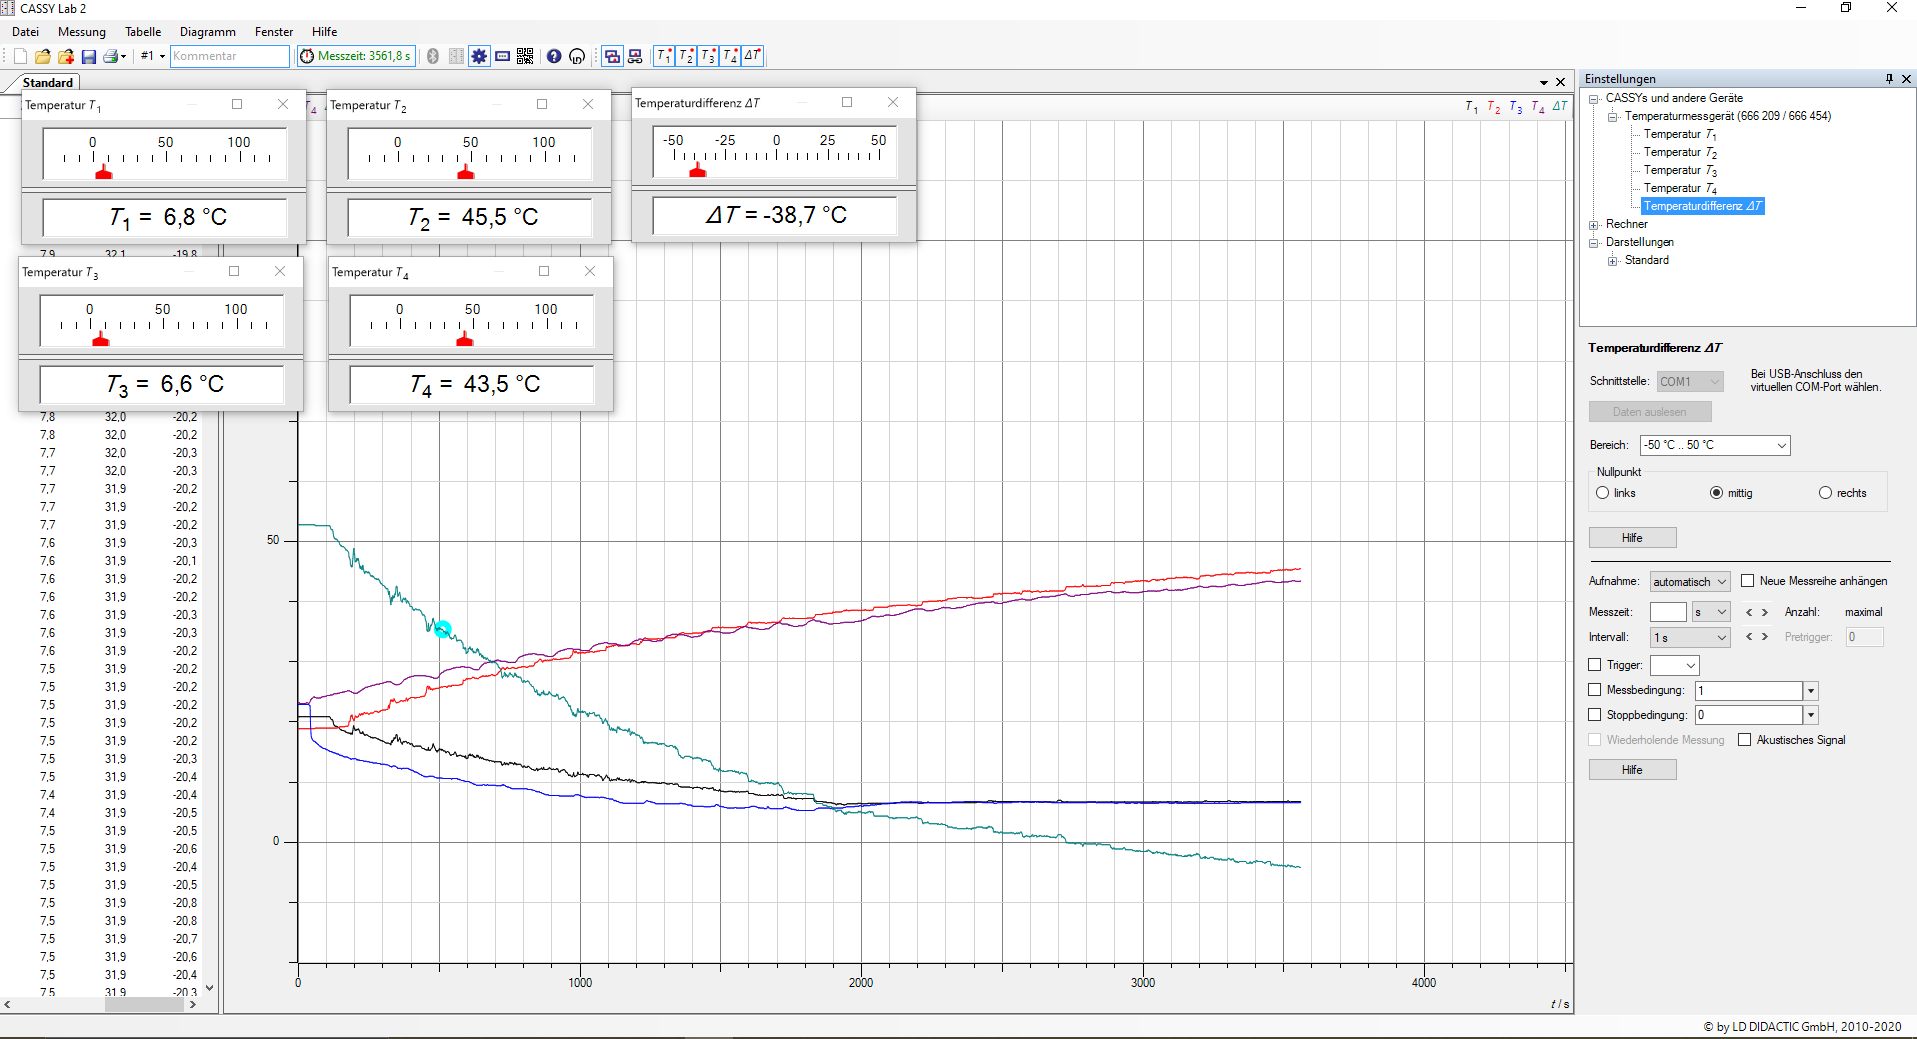
\includegraphics[width =\textwidth]{./figures/interface.PNG}
	\end{center}
	\caption{sichtbares Interface
	}\label{fig:interface}
\end{figure}

Nun wird der Kompressor (\SI{118(2)}{\watt}) an den Strom angeschlossen und
gleichzeitig die Aufzeichnung der Daten über den entsprechenden Knopf
gestartet. Zusätzlich zur Temperaturmessung werden ca.\ im 2 Minuten- Takt die
Drücke von den entsprechenden Barometern abgelesen, was in folgender
\autoref{tab:drucke} sichtbar ist. Um sicherzustellen, dass die Drücke die
richtige Zeit zugeordnet bekommen, werden Fotos von den Barometern gemacht und
mithilfe der erfassten Metadaten des Smartphones die genaue Zeit notiert.

\begin{table}[H]
	\caption[Abgelesene Drücke bei der entsprechenden Zeit]{Abgelesene Drücke bei der
		entsprechenden Zeit                                            \\
		$t$ \dots vergangene Zeit seit dem Start des Messvorgangs in s \\
		$p_k$ \dots abgelesener Druck auf der kalten Seite in bar      \\
		$p_w$ \dots abgelesener Druck auf der heißen Seite in bar
	}\label{tab:drucke}
	\centering
	\begin{tblr}{colspec={S[table-format=4.0(1)]S[table-format=1.2(2)]S[table-format=2.2(2)]}}
{{{$t$ / \si{\second}}}} & {{{$p_k$ / \si{\bar}}}} & {{{$p_w$ / \si{\bar}}}}\\
0(2) & 3.20(10) & 6.60(10)\\
115(2) & 3.20(10) & 7.00(10)\\
248(2) & 3.10(10) & 7.70(10)\\
383(2) & 2.65(10) & 8.20(10)\\
520(2) & 2.60(10) & 8.60(10)\\
650(2) & 2.40(10) & 9.00(10)\\
777(2) & 2.50(10) & 9.50(10)\\
909(2) & 2.10(10) & 9.80(10)\\
1034(2) & 2.05(10) & 10.20(10)\\
1156(2) & 1.90(10) & 10.45(10)\\
1280(2) & 1.90(10) & 10.80(10)\\
1403(2) & 1.80(10) & 11.00(10)\\
1530(2) & 1.75(10) & 11.40(10)\\
1650(2) & 1.75(10) & 11.60(10)\\
1770(2) & 1.70(10) & 11.80(10)\\
1915(2) & 1.80(10) & 11.75(10)\\
2035(2) & 1.90(10) & 12.20(10)\\
2156(2) & 1.90(10) & 12.80(10)\\
2278(2) & 1.90(10) & 12.50(10)\\
2408(2) & 1.85(10) & 13.40(10)\\
2531(2) & 1.85(10) & 13.20(10)\\
2653(2) & 1.85(10) & 13.90(10)\\
2779(2) & 1.85(10) & 14.00(10)\\
2899(2) & 1.85(10) & 13.90(10)\\
3022(2) & 1.80(10) & 14.30(10)\\
3144(2) & 1.80(10) & 14.60(10)\\
3264(2) & 1.80(10) & 14.80(10)\\
3390(2) & 1.80(10) & 15.00(10)\\
3513(2) & 1.80(10) & 15.00(10)\\
3632(2) & 1.80(10) & 15.20(10)\\
3753(2) & 1.80(10) & 15.60(10)\\
\end{tblr}

\end{table}

\subsection{Kennlinien und Kenndaten von Solarzellen bei Bestrahlung}

Nachdem die Solarzelle und die Lampe, wie bereits in
\autoref{sec:versuchsanordnung} sichtbar, aufgestellt sind, wird zunächst der
Abstand zwischen diesen bestimmt. Dieser beträgt \SI{284(5)}{\mm}. Die
Unsicherheit ist so groß gewählt, weil sich vor der Lampe eine gekrümmte
Glasplatte befindet, die die genaue Distanzmessung nicht erleichtert.
Zusätzlich sei angemerkt, dass die genaue Distanz zwischen jener Glasplatte und
der eigentlichen Glühbirne der Lampe nicht bekannt ist. Weiters fällt auf, dass
die Solarzellen nicht genau Parallel zu der Lampe angeordnet sind. Für diese
Verdrehung wird ein Winkel von \SI{5.0(1.0)}{\degree} gemessen. Auf diese
Verdrehung wird später in der \autoref{sec:diskussion} noch genauer
eingegangen.

Zusätzlich wird auch die Größe eines Solarzellenmoduls gemessen um die Fläche
bestimmen zu können. Der besseren Übersicht halber, werden diese Daten der
Aufzählung in \cref{list:flaechenSolar1} beigefügt.

\subsubsection{Serienschaltung der beiden Solarzellen}

Zunächst werden die Solarzellenmodule, wie in \autoref{fig:Serienschaltung}
sichtbar, in den Schaltplan integriert.

Nun wird der Widerstand mithilfe des, dafür vorgesehenen Reglers, variiert und
die abgelesenen Werte der Messgeräte in folgender
\autoref{tab:werte_serienschaltung} aufgelistet.

\begin{table}[]
	\caption[Abgelesene Strom und Spannungswerte für die Serienschaltung der
		Solarzellenmodule] {Abgelesene Strom und Spannungswerte für die Serienschaltung
		der Solarzellenmodule                        \\
		$U$ \dots Abgelesener Wert der Spannung in V \\
		$I$ \dots Abgelesener Wert des Stroms in mA
	}\label{tab:werte_serienschaltung}
	\centering
	\begin{tblr}{colspec={S[table-format=2.3(2)]S[table-format=2.3(2)]}}
{{{$U$ / \si{\volt}}}} & {{{$I$ / \si{\milli\ampere}}}}\\
12.03(3) & 0.000(3)\\
11.88(2) & 12.18(13)\\
11.83(2) & 14.14(15)\\
11.76(2) & 16.36(17)\\
11.72(2) & 18.08(19)\\
11.66(2) & 20.5(3)\\
11.60(2) & 23.0(3)\\
11.53(2) & 25.8(3)\\
11.46(2) & 28.9(3)\\
11.39(2) & 31.9(4)\\
11.34(2) & 33.8(4)\\
11.280(19) & 35.9(4)\\
11.240(19) & 37.5(4)\\
11.190(19) & 39.5(4)\\
11.140(19) & 41.0(5)\\
11.090(19) & 43.0(5)\\
11.040(19) & 44.6(5)\\
10.990(19) & 46.2(5)\\
10.930(19) & 48.1(5)\\
10.890(19) & 49.6(5)\\
10.810(19) & 52.1(6)\\
10.730(19) & 54.6(6)\\
10.660(18) & 56.3(6)\\
10.570(18) & 58.9(6)\\
10.480(18) & 61.2(7)\\
10.320(18) & 65.0(7)\\
10.120(18) & 67.8(7)\\
9.730(17) & 69.8(8)\\
9.680(17) & 70.3(8)\\
7.870(14) & 71.4(8)\\
5.680(11) & 72.3(8)\\
4.140(9) & 73.4(8)\\
2.880(7) & 75.2(8)\\
0.000(2) & 76.6(8)\\
\end{tblr}

\end{table}

Zusätzlich werden noch die Werte bei Leerlauf und einem simulierten Kurzschluss
gemessen. Dies geschieht, indem der Stromkreis zunächst geöffnet und dann ohne
Widerstand geschlossen wird. Der besseren Übersicht halber, sind diese Werte
auch in \autoref{tab:werte_serienschaltung} beigefügt.

\subsubsection{Parallelschaltung der beiden Solarzellen}
Auch bei der Parallelschaltung der beiden Solarzellen werden die Messwerte für
den variierenden Widerstand und für den Leerlauf, sowie den Kurzschluss, von
den Geräten abgelesen und in \autoref{tab:werte_parallelschaltung} aufgelistet.

\begin{table}[H]
	\caption[Abgelesene Strom und Spannungswerte für die Parallelschaltung der
		Solarzellenmodule] {Abgelesene Strom und Spannungswerte für die
		Parallelschaltung der Solarzellenmodule      \\
		$U$ \dots Abgelesener Wert der Spannung in V \\
		$I$ \dots Abgelesener Wert des Stroms in mA
	}\label{tab:werte_parallelschaltung}
	\centering
	\begin{tblr}{cells={font=\footnotesize},colspec={S[table-format=1.3(2)]S[table-format=3.3(3)]}}
{{{$U$ / \si{\volt}}}} & {{{$I$ / \si{\milli\ampere}}}}\\
5.760(11) & 0.000(3)\\
5.840(11) & 5.99(7)\\
5.830(11) & 6.68(7)\\
5.820(11) & 7.80(9)\\
5.810(11) & 10.14(11)\\
5.800(11) & 11.74(13)\\
5.770(11) & 17.32(18)\\
5.750(11) & 22.3(3)\\
5.720(11) & 29.0(3)\\
5.700(11) & 34.2(4)\\
5.670(11) & 40.7(5)\\
5.640(11) & 46.9(5)\\
5.620(11) & 52.3(6)\\
5.560(11) & 65.0(7)\\
5.510(11) & 76.7(8)\\
5.470(11) & 84.5(9)\\
5.410(11) & 96(1)\\
5.340(11) & 109.2(11)\\
5.28(1) & 120.6(13)\\
5.19(1) & 135.3(14)\\
5.04(1) & 153.8(16)\\
4.660(9) & 191(2)\\
4.550(9) & 196(2)\\
4.170(9) & 206(3)\\
3.620(8) & 207(3)\\
3.090(7) & 207(3)\\
2.510(6) & 208(3)\\
1.680(5) & 208(3)\\
1.080(4) & 209(3)\\
0.330(3) & 209(3)\\
0.000(2) & 211(3)\\
\end{tblr}

\end{table}

\subsubsection{Serienschaltung der beiden Solarzellen, wobei eine Solarzelle partiell abgeschattet wird}\label{list:flaechenSolar1}
Zunächst wird die Größe vermessen, die durch das Blatt Papier verdeckt ist, wie
in \autoref{fig:abgedeckt} sichtbar. Die entsprechenden Maße sind gemeinsam,
mit den anfangs gemessenen Werten der Solarzelle in folgender Aufzählung
angeführt.

\begin{enumerate}
	\item Fläche ganz: $\SI{10.0(2)}{\cm}\cdot \SI{8.0(2)}{\cm}=\SI{80(3)}{\cm\squared}$
	\item Fläche bedeckt: $\SI{10.0(2)}{\cm}\cdot
		      \SI{7.0(2)}{\cm}=\SI{70(3)}{\cm\squared}$
\end{enumerate}

Nun wird die gesamte Messung, wie bereits erklärt, für die verschiedenen
Widerstände, den Leerlauf und den Kurzschluss durchgeführt und die Messwerte in
\autoref{tab:werte_abgedeckt} aufgelistet.

\begin{table}[H]
	\caption[Abgelesene Strom und Spannungswerte für die Serienschaltung mit einem
		abgedeckten Solarzellenmodul] {Abgelesene Strom und Spannungswerte für die
		Serienschaltung mit einem abgedeckten Solarzellenmodul \\
		$U$ \dots Abgelesener Wert der Spannung in V           \\
		$I$ \dots Abgelesener Wert des Stroms in mA
	}\label{tab:werte_abgedeckt}
	\centering
	\begin{tblr}{cells={font=\footnotesize},colspec={S[table-format=2.3(2)]S[table-format=1.3(1)]}}
{{{$U$ / \si{\volt}}}} & {{{$I$ / \si{\milli\ampere}}}}\\
11.45(2) & 0.000(3)\\
6.540(12) & 6.68(7)\\
5.610(11) & 6.79(8)\\
5.360(11) & 6.84(8)\\
4.85(1) & 6.92(8)\\
4.090(9) & 7.02(8)\\
3.760(8) & 7.04(8)\\
3.470(8) & 7.06(8)\\
2.930(7) & 7.11(8)\\
2.500(6) & 7.14(8)\\
2.100(6) & 7.20(8)\\
1.660(5) & 7.30(8)\\
1.470(5) & 7.34(8)\\
0.990(4) & 7.44(8)\\
0.670(4) & 7.55(8)\\
0.390(3) & 7.63(8)\\
0.490(3) & 7.68(8)\\
0.190(3) & 7.69(8)\\
0.000(2) & 7.65(8)\\
\end{tblr}

\end{table}

\subsection{Diodenparameter und Wirkungsgrad einer Solarzelle}

\subsubsection{Messung der Dunkelkennlinie}

Zunächst wird die Solarzelle komplett abgedunkelt. Dazu wird diese vollflächig
mit einem Stück Papier abgedeckt. Zusätzlich wird dieses Papier mit einem
schwereren Gegenstand beschwert, um dafür zu sorgen, dass die Solarzelle
wirklich vollflächig abgedeckt ist.

Um die Diodenkennlinie aufzuzeichnen, wird das Sourcemeter mit dem Rechner
verbunden und das Programm, Kickstart geöffnet. Nun wird in der entsprechenden
Software unter dem Menüpunkt \dq new\dq \ eine neue Messung gestartet. Nach
erfolgreicher Verbindung mit dem Sourcemeter 2450 und der eingabe aller
Parameter, wie z.B.\ den Maximalen Strom, wie in den Unterlagen aus
\cite{knoll_solarzelle_nodate} beschrieben, kann die Messung gestartet werden.
Die so erzeugte Diodenkennlinie ist in \autoref{fig:mess_dunkelkennlinie}
sichtbar.

\begin{figure}[H]
	\centering
	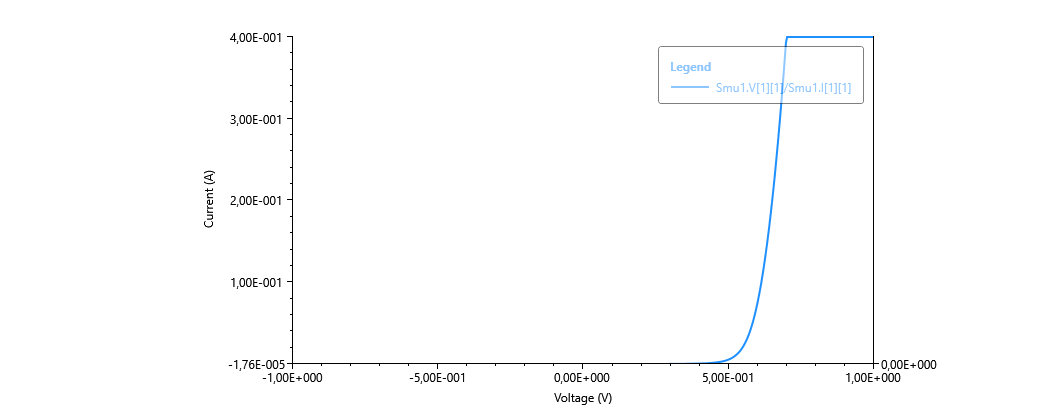
\includegraphics[width=0.95\textwidth]{figures/dunekl.png}
	\caption{Erzeugte Dunkelkennlinie der Solarzelle
	}\label{fig:mess_dunkelkennlinie}
\end{figure}

\subsubsection{Messung der Hellkennlinie und Bestimmung des Wirkungsgrades}

Nun werden die Lampen, wie bereits in \autoref{sec:versuchsanordnung}
beschrieben, positioniert und ebenfalls die Kennlinien aufgenommen. Die
entsprechende Leistung der Lichtquelle wird anhand des Sensors bestimmt und vom
analogen Messgerät abgelesen, was gemeinsam mit den entsprechenden Größen in
folgender Aufzählung in \Cref{enum:werte_solarzelle2} ersichtlich ist. Auch die
Diodenkennlinien für die verschiedenen Lampen werden, wie zuvor die
Dunkelkennlinie, aufgenommen und sind in den folgenden
\autoref{fig:mess_hellkennlinie_lampe} bis \autoref{fig:mess_hellkennlinie_led}
sichtbar.

\begin{enumerate}\label{enum:werte_solarzelle2}
	\item Durchmesser des Sensors: $\SI{1.80(5)}{\cm}$\cite{noauthor_2450_nodate}
	\item Fläche der Solarzelle: $\SI{1.70(10)}{\cm}\cdot \SI{3.90(10)}{\cm}$
	\item Strahlungsfluss Lampe Messung 1: $\SI{63(2)}{\milli\watt}$
	\item Strahlungsfluss Lampe Messung 2: $\SI{106(3)}{\milli\watt}$
	\item Strahlungsfluss LED Messung 2: $\SI{264(3)}{\milli\watt}$
\end{enumerate}

\begin{figure}[H]
	\centering
	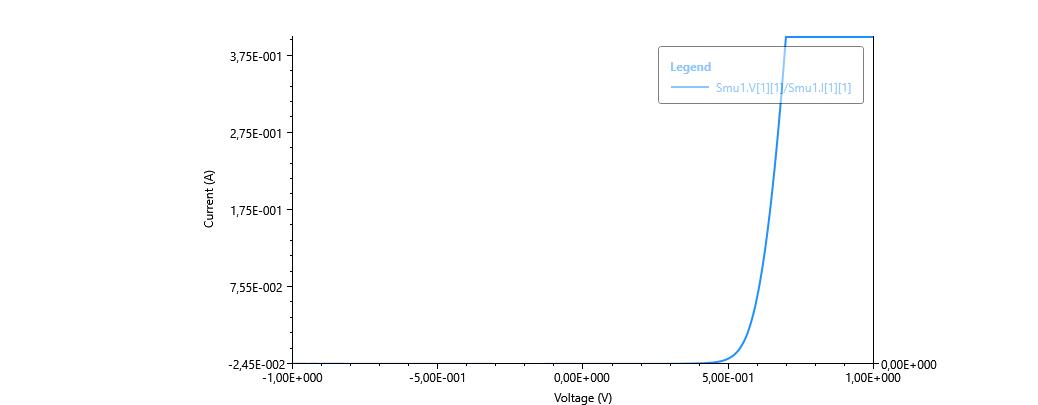
\includegraphics[width=0.95\textwidth]{figures/helllampe.png}
	\caption{Erzeugte Diodenkennlinie für die Halogenlampe
	}\label{fig:mess_hellkennlinie_lampe}
\end{figure}

\begin{figure}[H]
	\centering
	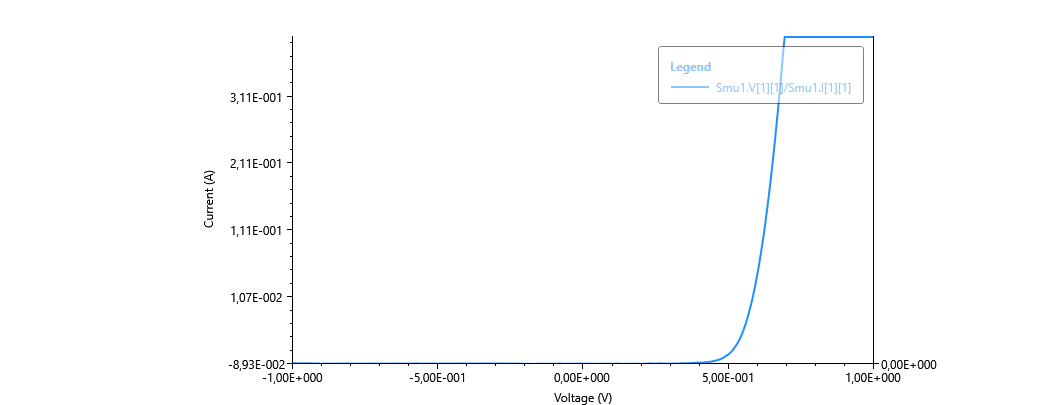
\includegraphics[width=0.95\textwidth]{figures/helllampe2.png}
	\caption{Erzeugte Diodenkennlinie für die Halogenlampe mit geringeren Abstand zur Solarzelle
	}\label{fig:mess_hellkennlinie_lampe2}
\end{figure}

\begin{figure}[H]
	\centering
	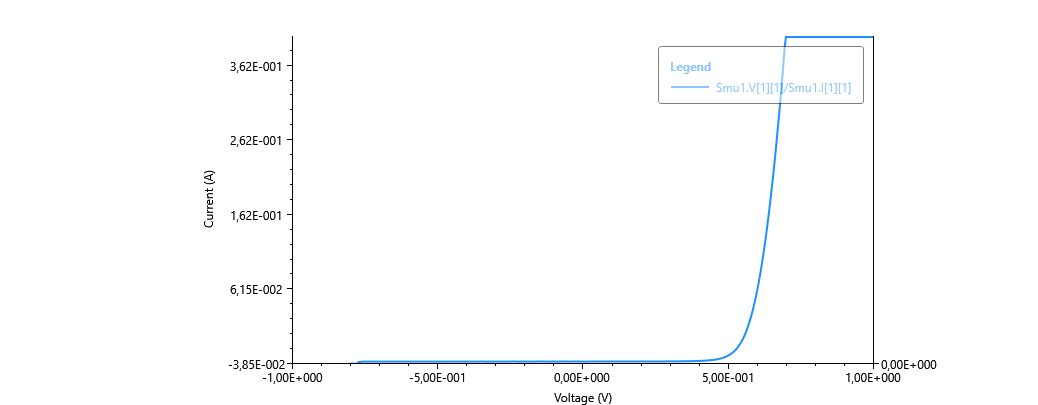
\includegraphics[width=0.95\textwidth]{figures/hellled.png}
	\caption{Erzeugte Diodenkennlinie für die LED-Lampe
	}\label{fig:mess_hellkennlinie_led}
\end{figure}

\section{Auswertung}\label{sec:auswertung}

Um zu sehen wie sich die Unsicherheit der Messungen bis in die Ergebnisse
fortpflanzt, ist erweiterte Gauss-Methode verwendet worden. Die Grundlagen
dieser Methode stammen von den Powerpointfolien von
GUM~\cite{wolfgang_kessel_isobipm-gum_2004}. Für die Auswertung ist die
Progammiersprache Python im speziellen die Pakete \verb#labtool-ex2#,
\verb#pandas#, \verb#sympy#, \verb#lmfit# zur Hilfe genommen worden.
\verb#lmfit# wurde für das Fitten verwendet, \verb#sympy# wurde für symbolische
Manipulation verwendet und die restlichen Pakete für leichteres Handhaben der
Daten. Dies wurde aber alles durch \verb#labtool-ex2# abstrahiert.

Um höchstmögliche Genauigkeit zu garantieren wird erst bei der Darstellung der
Wert in Tabellen gerundet.

\subsection{Wärmepumpe}

Zunächst gilt es die zeitlichen Temperatur und Druckverläufe des kalten und des
warmen Bereich darzustellen dazu sind die Daten in zwei Diagrammen geplottet
worden. Dies ist gemacht worden um zeitliche Tendenzen besser zu präsentieren.

\begin{figure}[H]
	\centering
	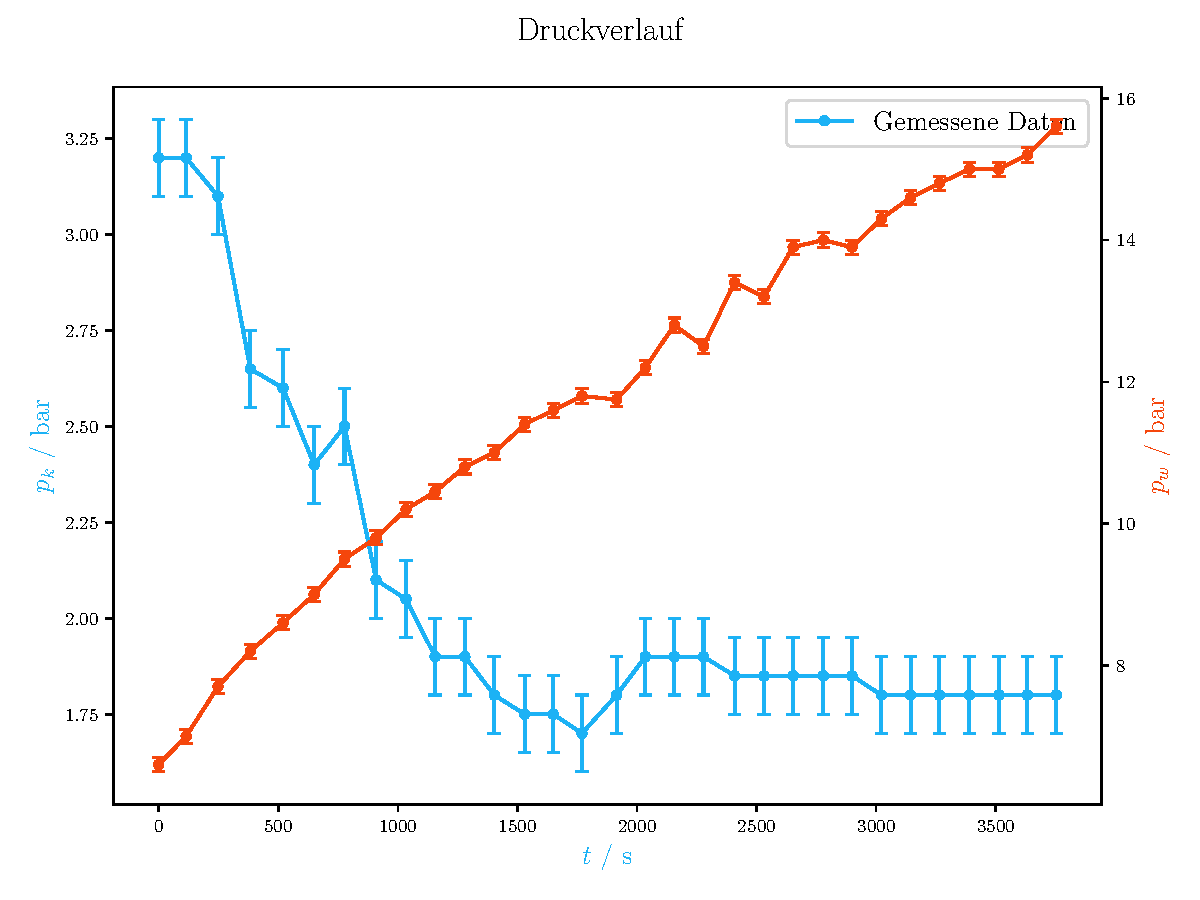
\includegraphics[width=0.49\textwidth]{figures/pressureProfile.pdf}
	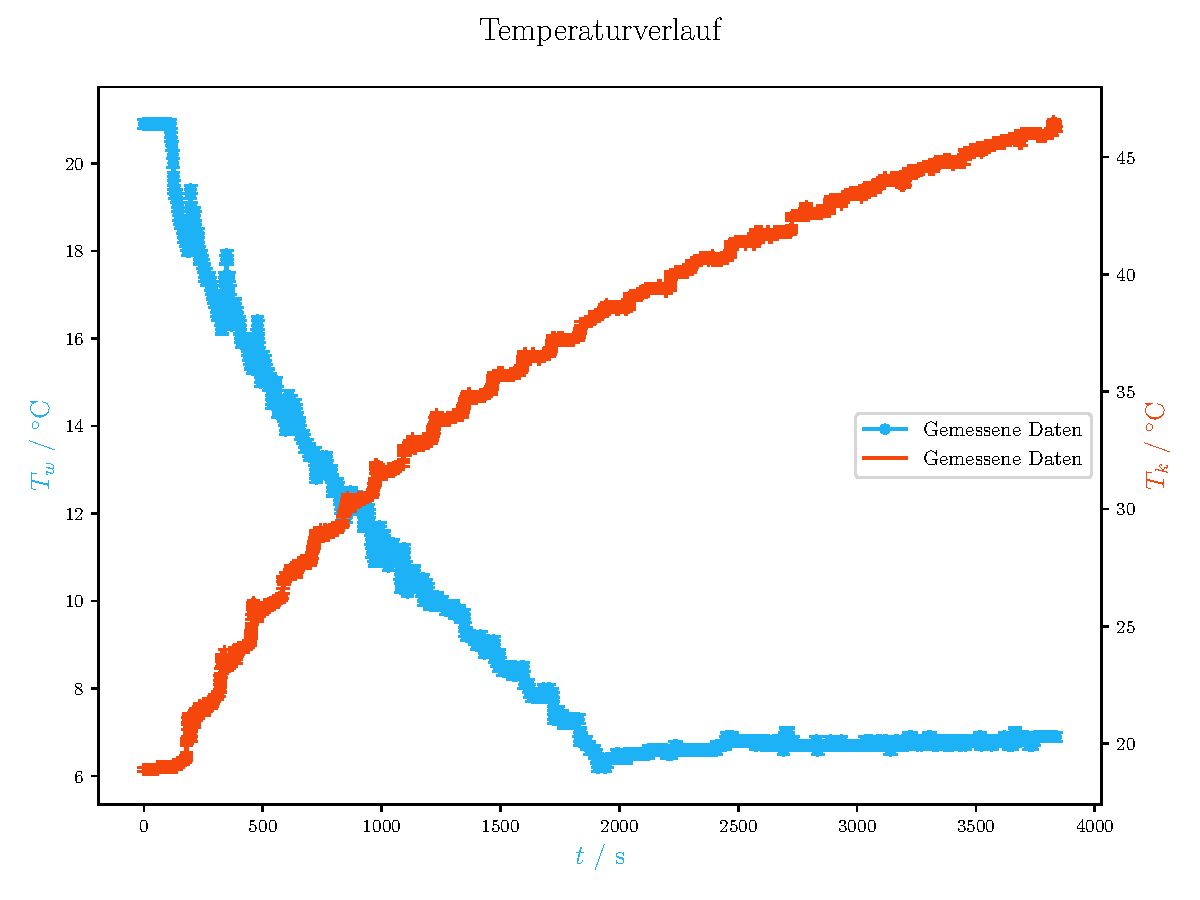
\includegraphics[width=0.49\textwidth]{figures/temperatureProfile.pdf}
	\caption[Zeitliche Verläufe von den Drücken und Temperaturen, während dem Betrieb der
		Wärmepumpe]{Zeitliche Verläufe von den Drücken und Temperaturen, während dem
		Betrieb der Wärmepumpe. Wobei $p_k$ der Druck und $T_k$ die Temperatur des
		Reservoirs der kalten Seite der Wärmepumpe sind. $p_w$ und $T_w$ sind
		dementsprechend, die der warmen Seite der Wärmepumpe.
	}\label{fig:druckTemperaturVerlauf}
\end{figure}

Nun wird mittels der zeitlichen Änderung der warmen Reservoir-Temperatur der
Wärmefluss mittels der Masse und Wärmekapazität des Reservoirs errechnet
${\dot{Q}= (m_1) c_w \Delta \dot{T}}$. Hier wurde die Warme Aufgrund des
stetigeren Temperaturverlaufs gewählt. Schlussendlich wird durch die zugeführte
elektrische Leistung dividiert um die Leistungszahl zu bekommen, siehe
\autoref{eq:Leistungszahl}.

\begin{figure}[H]
	\centering
	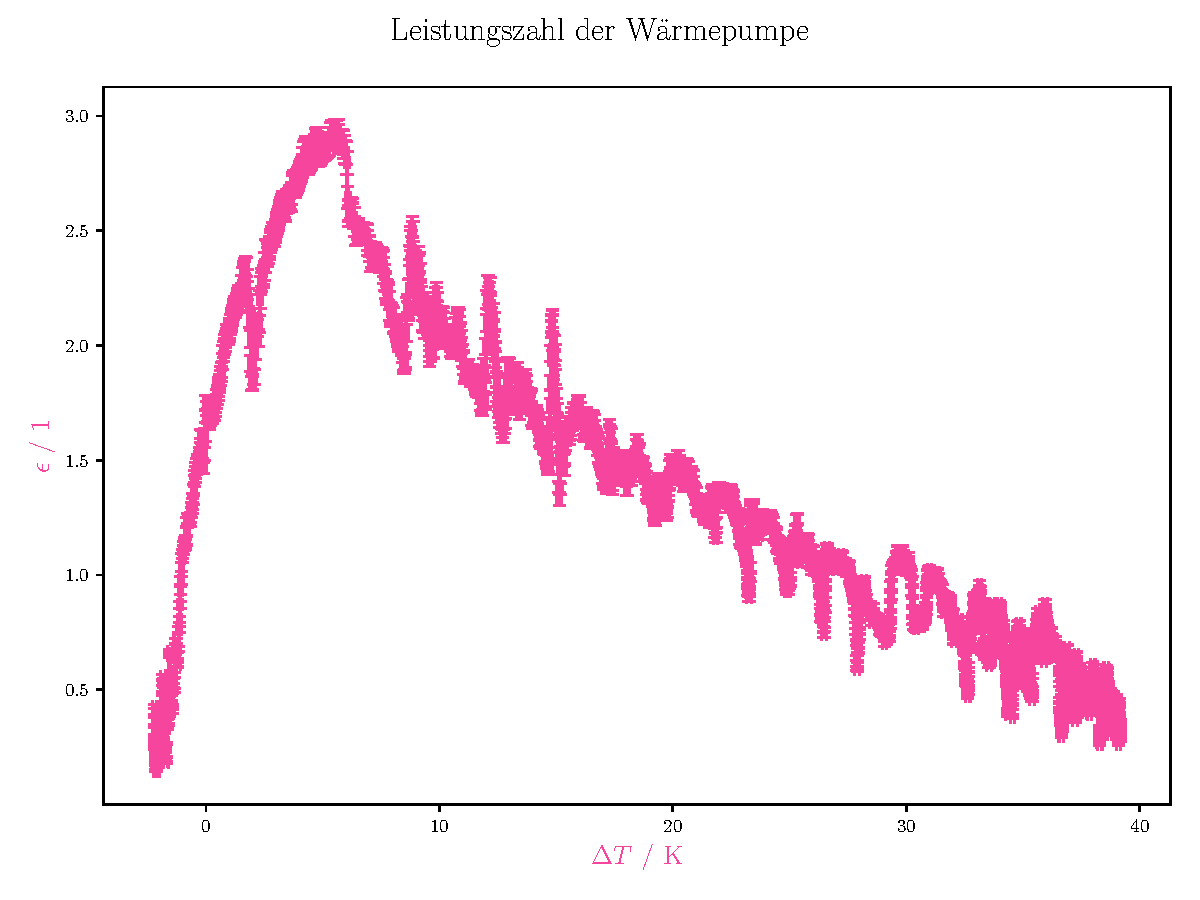
\includegraphics[width=0.95\textwidth]{figures/leistungszahlVerlauf.pdf}
	\caption[Verlauf der Leistungszahl]{Verlauf der Leistungszahl $\epsilon$ einer
		Wärmepumpe, während diese durch ihren Betrieb die Temperaturdifferenz der zwei
		Reservoirs $\Delta T$ erhöht.
	}\label{fig:leistungszahlVerlauf}
\end{figure}

Indem nun diese Leistungszahlen $\epsilon$ in Relation zu dem hier theoretisch
Maximalen $\epsilon_\text{max}$ gesetzt wird, kann der Gütefaktor $\eta$
bestimmt werden, wie in \autoref{eq:guetefaktor} sichtbar. Dabei wurde
$\epsilon_\text{max}$ durch den Kehrwert des Carnot-Wirkungsgrad bestimmt, die
höchst und tiefst Temperaturen sind aus den Daten genommen worden
${\epsilon_\text{max} = \frac{1}{1-\frac{T_k}{T_w}}}$.

\begin{figure}[H]
	\centering
	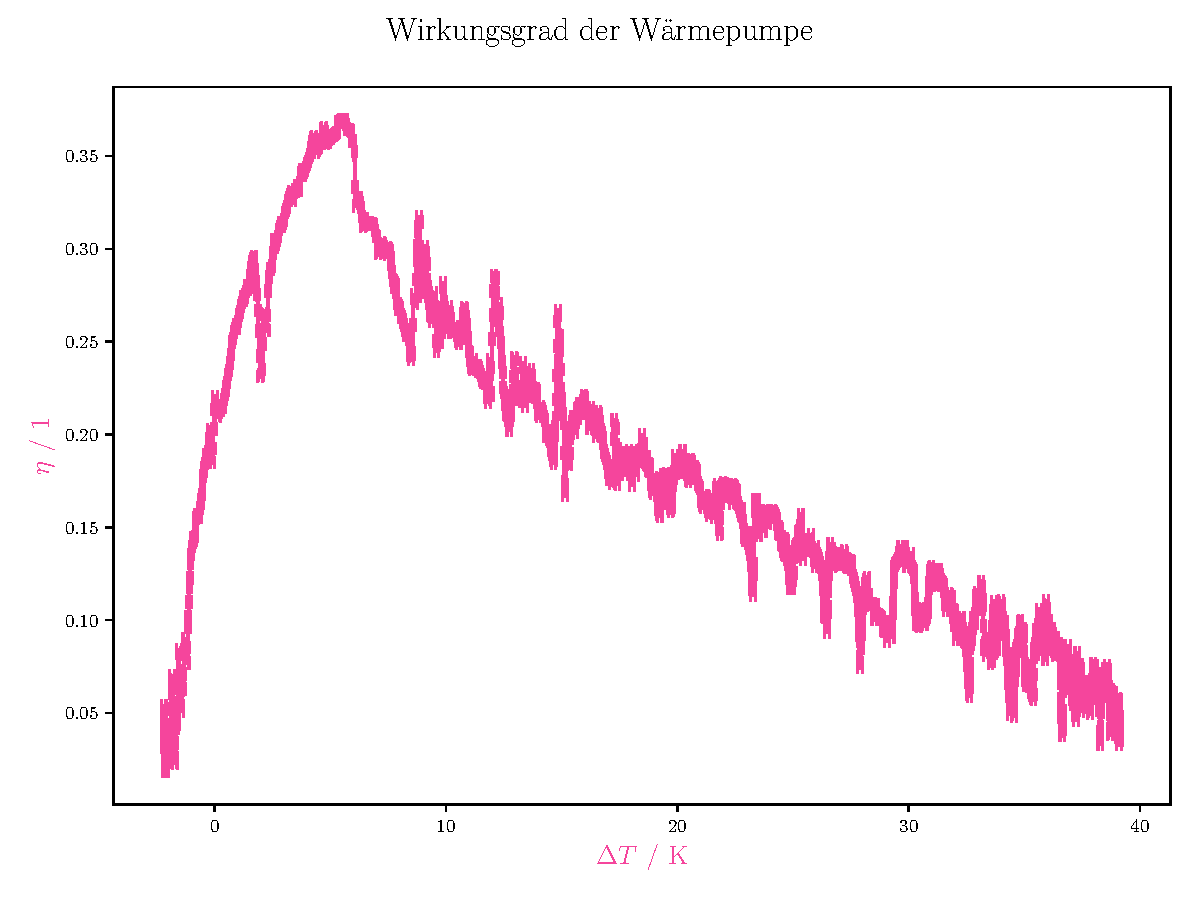
\includegraphics[width=0.95\textwidth]{figures/wirkungsgradVerlauf.pdf}
	\caption[Dynamischer Gütegradverlauf $\eta$ der Wärmepumpe]{Dynamischer Gütegradverlauf
		$\eta$ der Wärmepumpe. Der Gütegrad $\eta$ wird bezüglich der
		Temperaturdifferenz der zwei Reservoirs $\Delta T$ aufgetragen. Die, für diese
		Graphik errechnete, theoretisch maximale Leistungszahl $\epsilon_\text{max}$
		ist auch angeführt.
	}\label{fig:wirkungsgradVerlauf}
\end{figure}

\subsection{Kennlinien und Kenndaten von Solarzellen bei Bestrahlung}
Damit die invertierte Strom-Spannung Kennlinie und die Leistungskennlinie
leserlich bleiben sind diese in zwei nebeneinanderliegenden Plots gezeichnet

Um die Kenndaten zu erzeugen sind folgende Statistiken auf die Datensätze
angewandt worden. Damit der Kurzschlussstrom $I_k$ ermittelt werden kann ist
der Messwert bei der Spannung von $\SI{0}{\volt}$, für die Leerlaufspannung
$U_L$ der Messwert mit keinem Strom $\SI{0}{\ampere}$ genommen worden. Für den
Betriebspunkt der maximalen Leistung ist zunächst die Leistung mit $P=UI$
berechnet und von diesen Werten das Maximum genommen worden, um $P_\text{MPP}$
zu bestimmen, und die Spannung $U_\text{MPP}$ und Strom $I_\text{MPP}$, die
diese Leistung produzierten, vermerkt worden. Dieses Verfahren ist für die
verschiedenen Beschaltungen und Belichtungsflächen durchgeführt worden.

\subsubsection{Serienschaltung der beiden Solarzellen}
\begin{figure}[H]
	\centering
	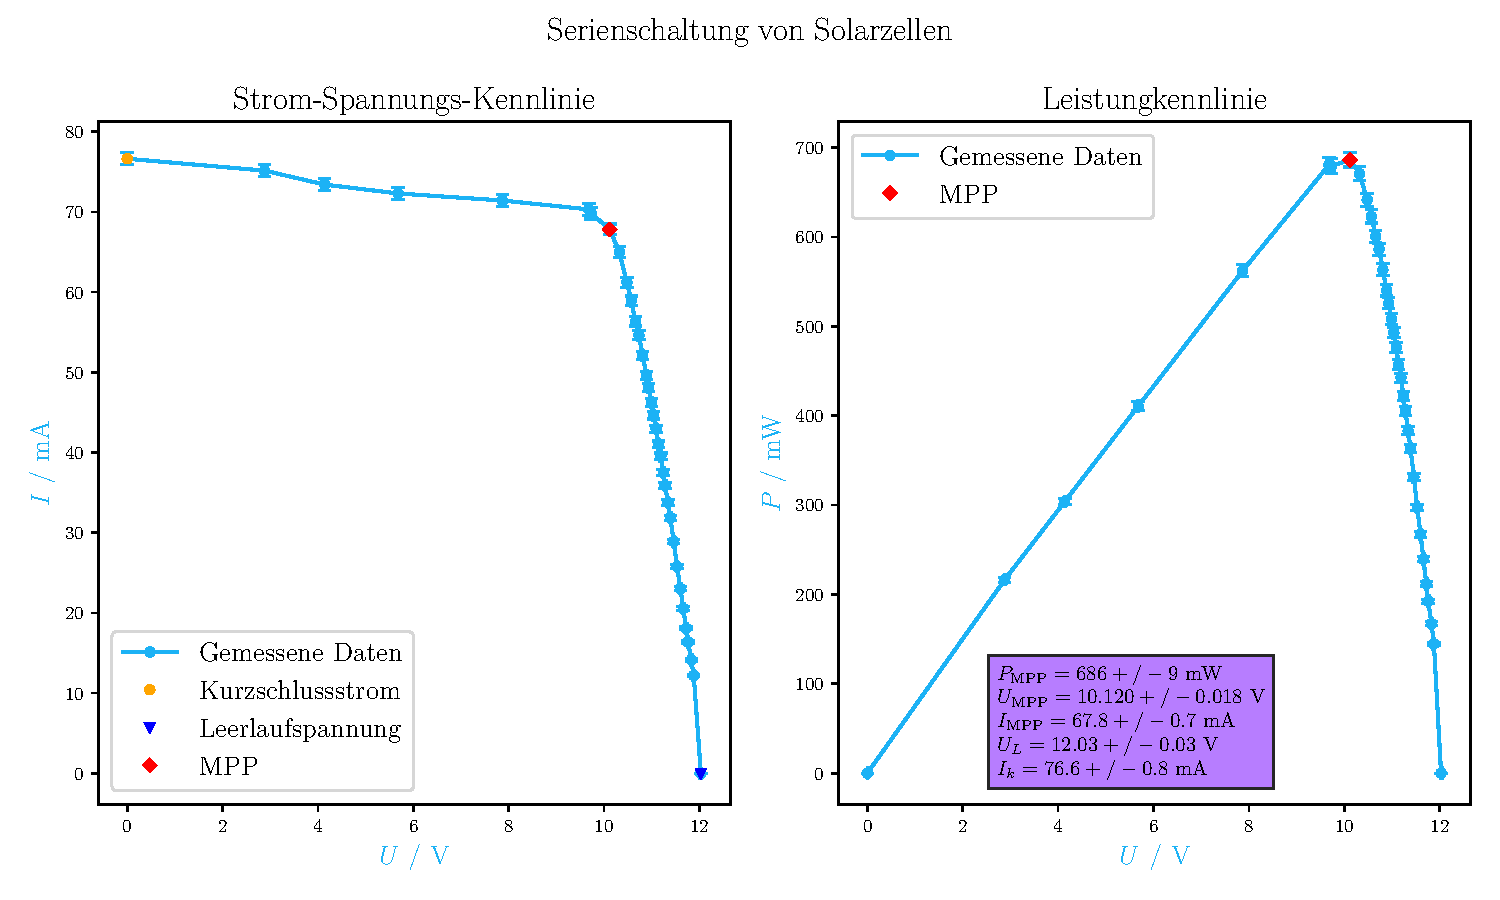
\includegraphics[width=0.95\textwidth]{figures/serienschaltung.pdf}
	\caption[Kennlinien Serienschaltung Solarzellen]{Untersuchung der invertierten
		Strom-Spannungs Kennlinie (links) und Leistungskennlinie (rechts) bei einer
		Serienschaltung von Solarzellen. Folgende Größen wurden errechnet und, um
		Effizienz für dieser Konfiguration besser vergleichen zu können, auch
		angeführt:                           \\
		$I_k \dots$ Kurzschlussstrom         \\
		$U_L \dots$ Leerlaufspannung         \\
		$P_\text{MPP} \dots$ Leistung am MPP \\
		$I_\text{MPP} \dots$ Strom am MPP    \\
		$U_\text{MPP} \dots$ Spannung am MPP \\
		$FF \dots$ Füllfaktor der Solarzellenkonfiguration
	}\label{fig:auws_kennlinie_serie}
\end{figure}

\subsubsection{Parallelschaltung der beiden Solarzellen}
\begin{figure}[H]
	\centering
	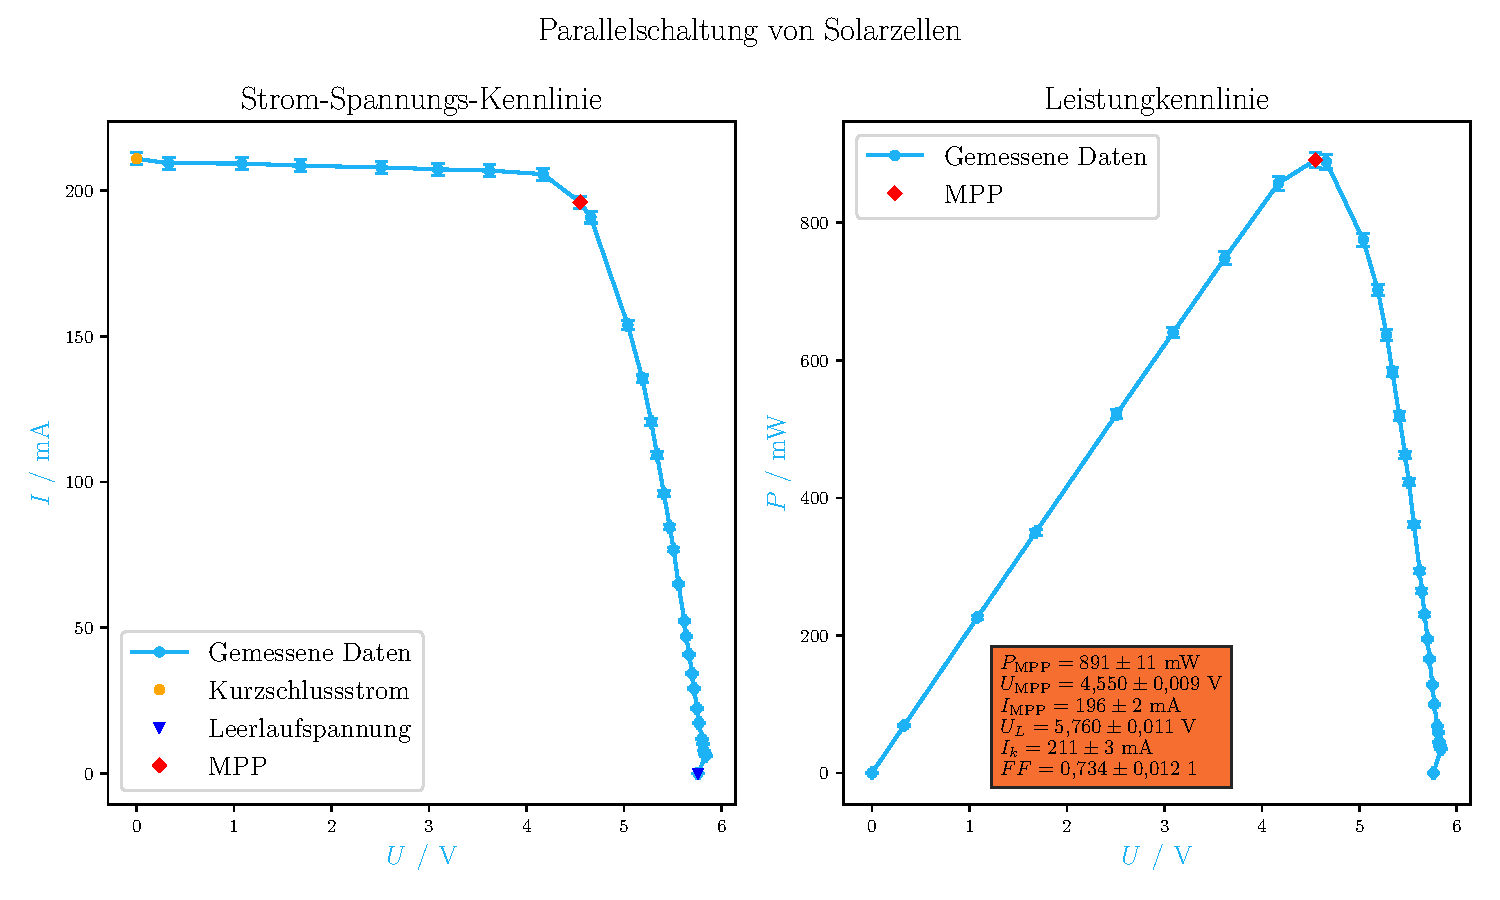
\includegraphics[width=0.95\textwidth]{figures/parallelschaltung.pdf}
	\caption[Kennlinien Parallelschaltung Solarzellen]{Untersuchung der invertierten
		Strom-Spannungs Kennlinie (links) und Leistungskennlinie (rechts) bei einer
		Parallelschaltung von Solarzellen. Folgende Größen wurden errechnet und, um
		Effizienz für dieser Konfiguration besser vergleichen zu können, auch
		angeführt:                           \\
		$I_k \dots$ Kurzschlussstrom         \\
		$U_L \dots$ Leerlaufspannung         \\
		$P_\text{MPP} \dots$ Leistung am MPP \\
		$I_\text{MPP} \dots$ Strom am MPP    \\
		$U_\text{MPP} \dots$ Spannung am MPP \\
		$FF \dots$ Füllfaktor der Solarzellenkonfiguration
	}\label{fig:auws_kennlinie_parallel}
\end{figure}

\subsubsection{Serienschaltung der beiden Solarzellen, wobei eine Solarzelle partiell abgeschattet wird}

\begin{figure}[H]
	\centering
	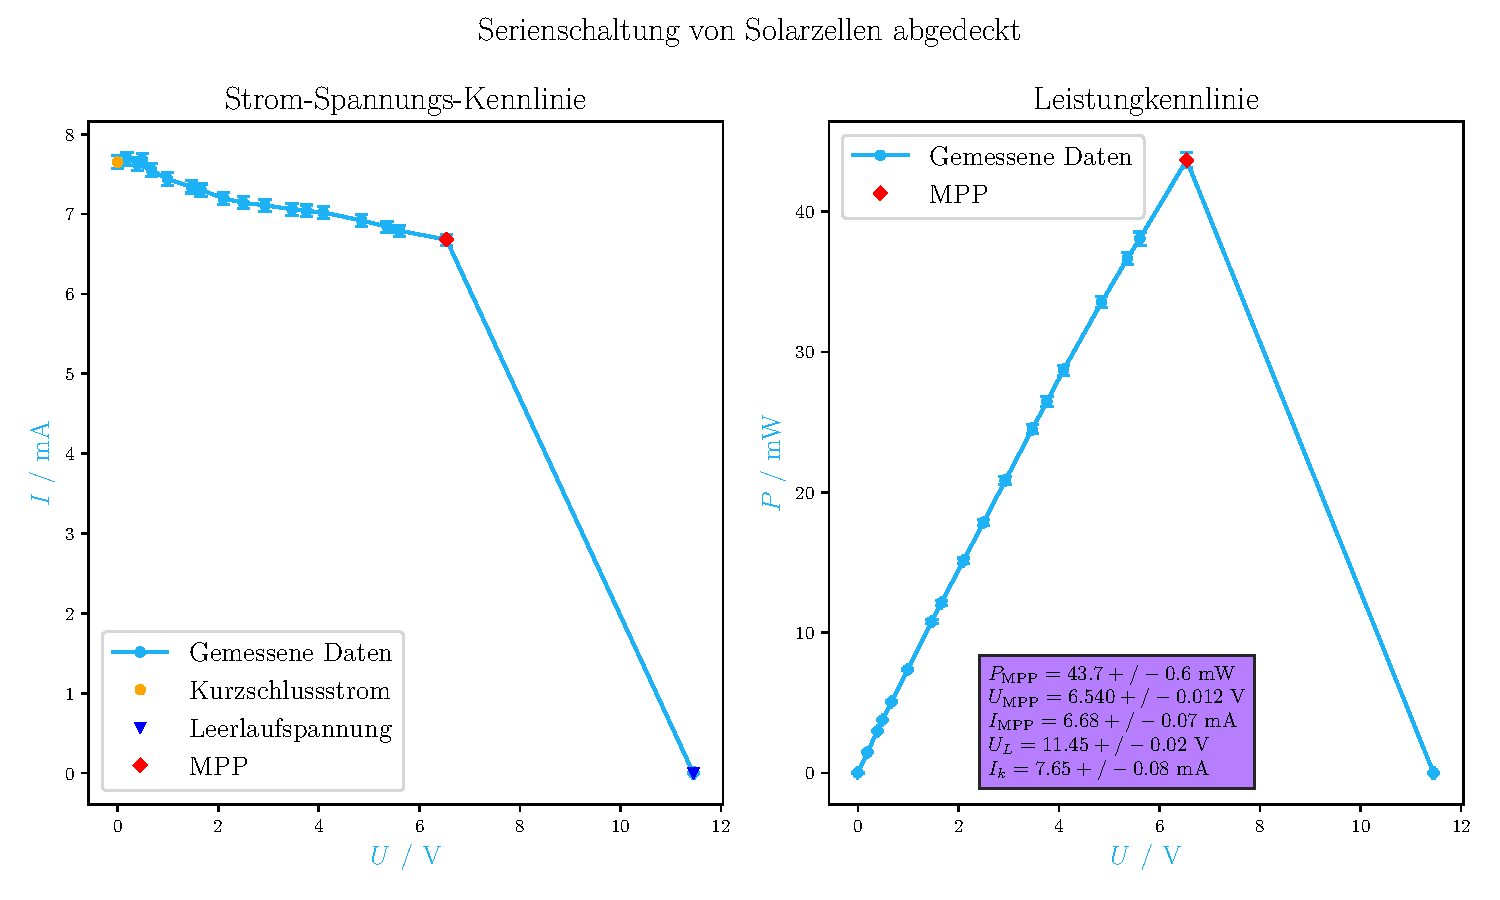
\includegraphics[width=0.95\textwidth]{figures/serienschaltungAbgedeckt.pdf}
	\caption[Kennlinien Serienschaltung mit teils bedeckten Solarzellen]{Untersuchung der
		invertierten Strom-Spannungs Kennlinie (links) und Leistungskennlinie (rechts)
		bei einer Serienschaltung mit Teilbedeckung der Solarzellen. Folgende Größen
		wurden errechnet und, um Effizienz für dieser Konfiguration besser vergleichen
		zu können, auch angeführt:           \\
		$I_k \dots$ Kurzschlussstrom         \\
		$U_L \dots$ Leerlaufspannung         \\
		$P_\text{MPP} \dots$ Leistung am MPP \\
		$I_\text{MPP} \dots$ Strom am MPP    \\
		$U_\text{MPP} \dots$ Spannung am MPP \\
		$FF \dots$ Füllfaktor der Solarzellenkonfiguration
	}\label{fig:auws_kennlinie_abgedeckt}
\end{figure}

\subsection{Diodenparameter und Wirkungsgrad einer Solarzelle}

Nun werden die Diodencharakteristik einer Solarzelle bei verschiedenen
Belichtungsstufen untersucht. Dazu wurde die Strom-Spannung Kennlinien gemessen
und an die Gleichung für das Zweidioden-Modell gefittet. Um dies zu
bewerkstelligen wurden folgende Vereinfachungen getroffen: Die implizite
Anteile werden vernachlässigt, was bewirkt dass die gefittet Funktion höher
sein wird als wenn die Terme berücksichtigt werden. Beim fitten war der zweite
Diodenparameter nahe 0 und deshalb wurde die Fit-Kurve nochmals vereinfacht und
dieser Term weggelassen. Somit wurde schlussendlich mit folgender Gleichung
gefittet:

\begin{equation}
	I(U) = I_{S1} \left( \exp{\frac{eU}{f_1 k_b T}} -1 \right) - I_{ph}
	\label{eq:kennlinienFit}
\end{equation}

Dabei ist $I_{S1}$ der Sättigungsstrom, $U$ die gemessene Spannung, $k_b$ die
Boltzmann-Konstante, $e$ die Elementar Ladung, $T$ die Temperatur der
Solarzelle, $f_1$ der Diodenfaktor und $I_{ph}$ der Photostrom.

Damit die Konvergenz der Parameter funktionieren konnte, wurde die Anzahl der
freien Parameter reduziert. Dafür wurde die Temperatur gewählt, welche am
besten abgeschätzt werden konnte. Weiters wurde, wegen demselben Grund, der
Cutoff Bereich von \SI{0.4}{\ampere} verworfen, da es nicht den echten Verlauf
wiederspiegelt.

\subsubsection{Messung der Dunkelkennlinie}

Nun wird die Dunkelkennlinie bestimmmt. Dabei wurden bei den aufgenommen Daten
die Werte mit einer Spannung unter \SI{0.15}{\volt} verworfen, da zunächst der
Tail zu großen Einfluss auf den Fit hatte. Die Kurve hat viel zu spät zum
Steigen begonnen und damit den dynamischen Teil nicht richtig beschrieben.
Deshalb wurde auch nur der interpolierte Bereich geplottet und es wurde nichts
extrapoliert.

\begin{figure}[H]
	\centering
	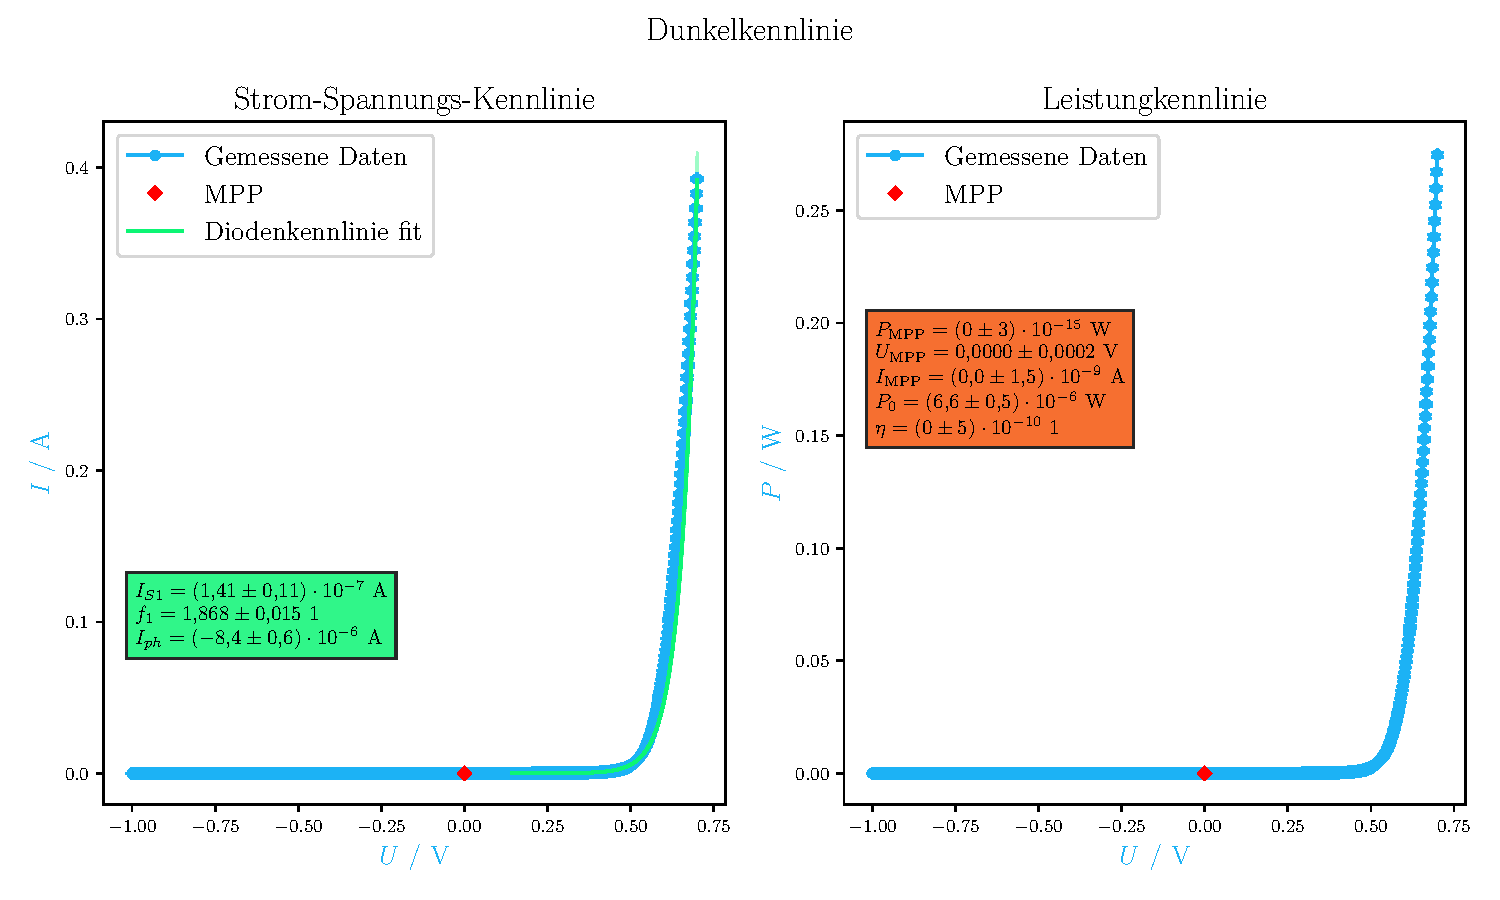
\includegraphics[width=0.95\textwidth]{figures/dunkelkennlinie.pdf}
	\caption[Dunkelkennlinie einer Solarzelle]{Untersuchung der Strom-Spannungs Kennlinie
		(links) und Leistungskennlinie (rechts) bei keiner Belichtung der Solarzelle.
		Folgende Größen wurden errechnet und, um Effizienz für dieser Konfiguration
		besser vergleichen zu können, auch angeführt: \\
		$P_\text{MPP} \dots$ Leistung am MPP          \\
		$I_\text{MPP} \dots$ Strom am MPP             \\
		$U_\text{MPP} \dots$ Spannung am MPP          \\
		$P_0 \dots$ Zugeführte Strahlungsfluss        \\
		$\eta \dots$ Wirkungsgrad
	}\label{fig:ausw_kennlinie_dunkel}
\end{figure}

\subsubsection{Messung der Hellkennlinie und Bestimmung des Wirkungsgrades}

Für die Hellkennlinien musst der Tail nicht weniger gewichtet werden, da die
Fits auch so zu einem sinnvollen Ergebnis konvergiert sind.

\begin{figure}[H]
	\centering
	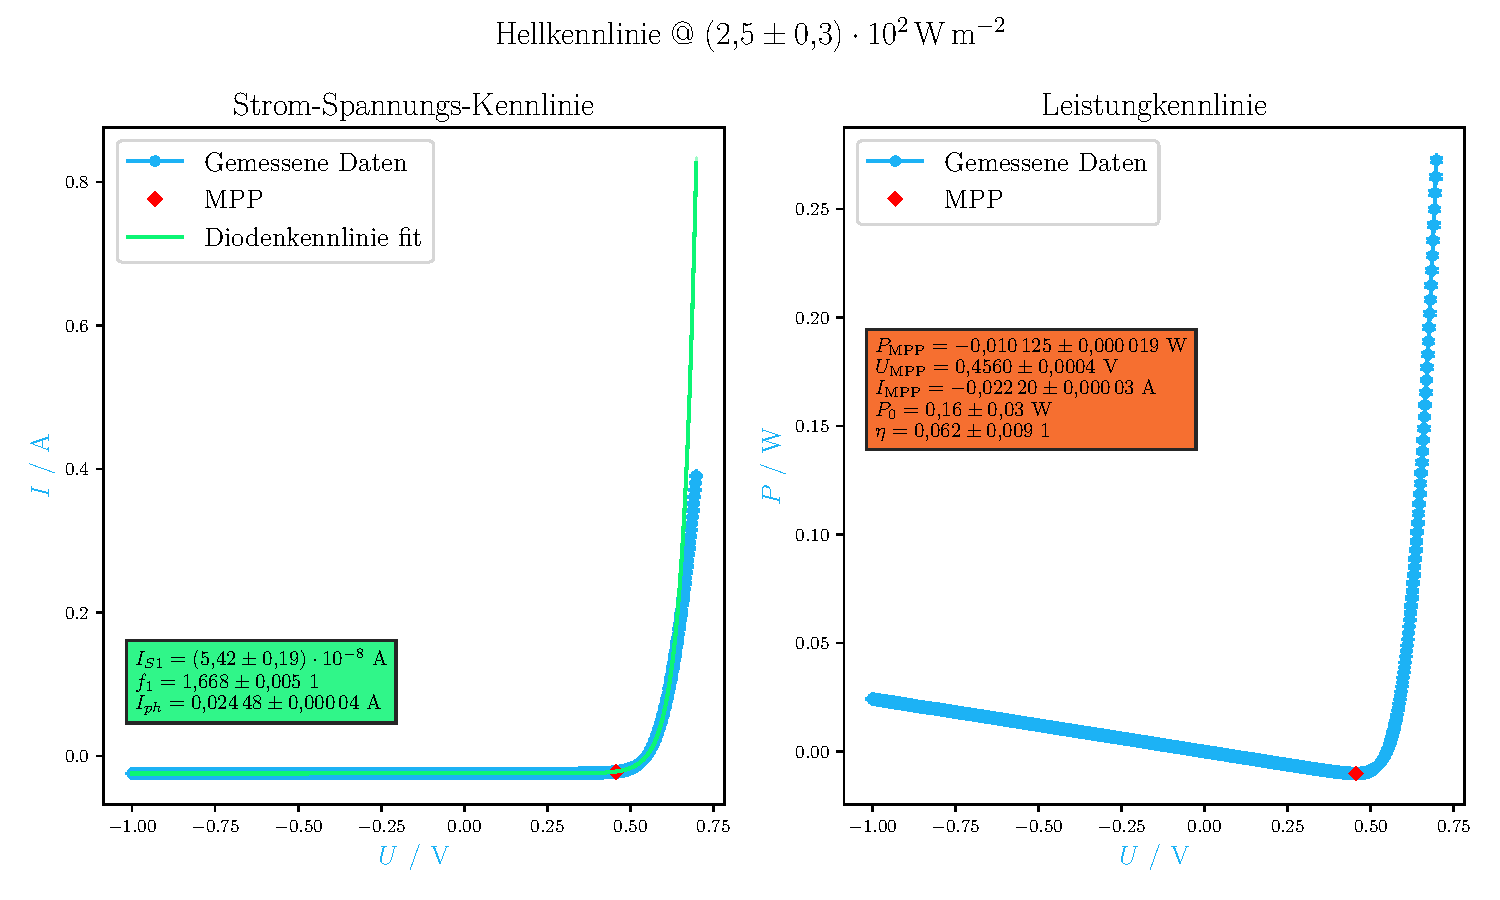
\includegraphics[width=0.95\textwidth]{figures/helllampe.pdf}
	\caption[Kennlinie durch Halogen-Lampen 1.te Belichtung]{Untersuchung der
		Strom-Spannungs Kennlinie (links) und Leistungskennlinie (rechts) bei einer
		Bestrahlungsstärke der Solarzelle von \SI{250(30)}{\watt\per\meter\squared}
		mittels einer Halogenlampe. Folgende Größen wurden errechnet und, um Effizienz
		für dieser Konfiguration besser vergleichen zu können, auch angeführt: \\
		$P_\text{MPP} \dots$ Leistung am MPP                                   \\
		$I_\text{MPP} \dots$ Strom am MPP                                      \\
		$U_\text{MPP} \dots$ Spannung am MPP                                   \\
		$P_0 \dots$ Zugeführte Strahlungsfluss                                 \\
		$\eta \dots$ Wirkungsgrad
	}\label{fig:ausw_kennlinie_hell_lampe}
\end{figure}

\begin{figure}[H]
	\centering
	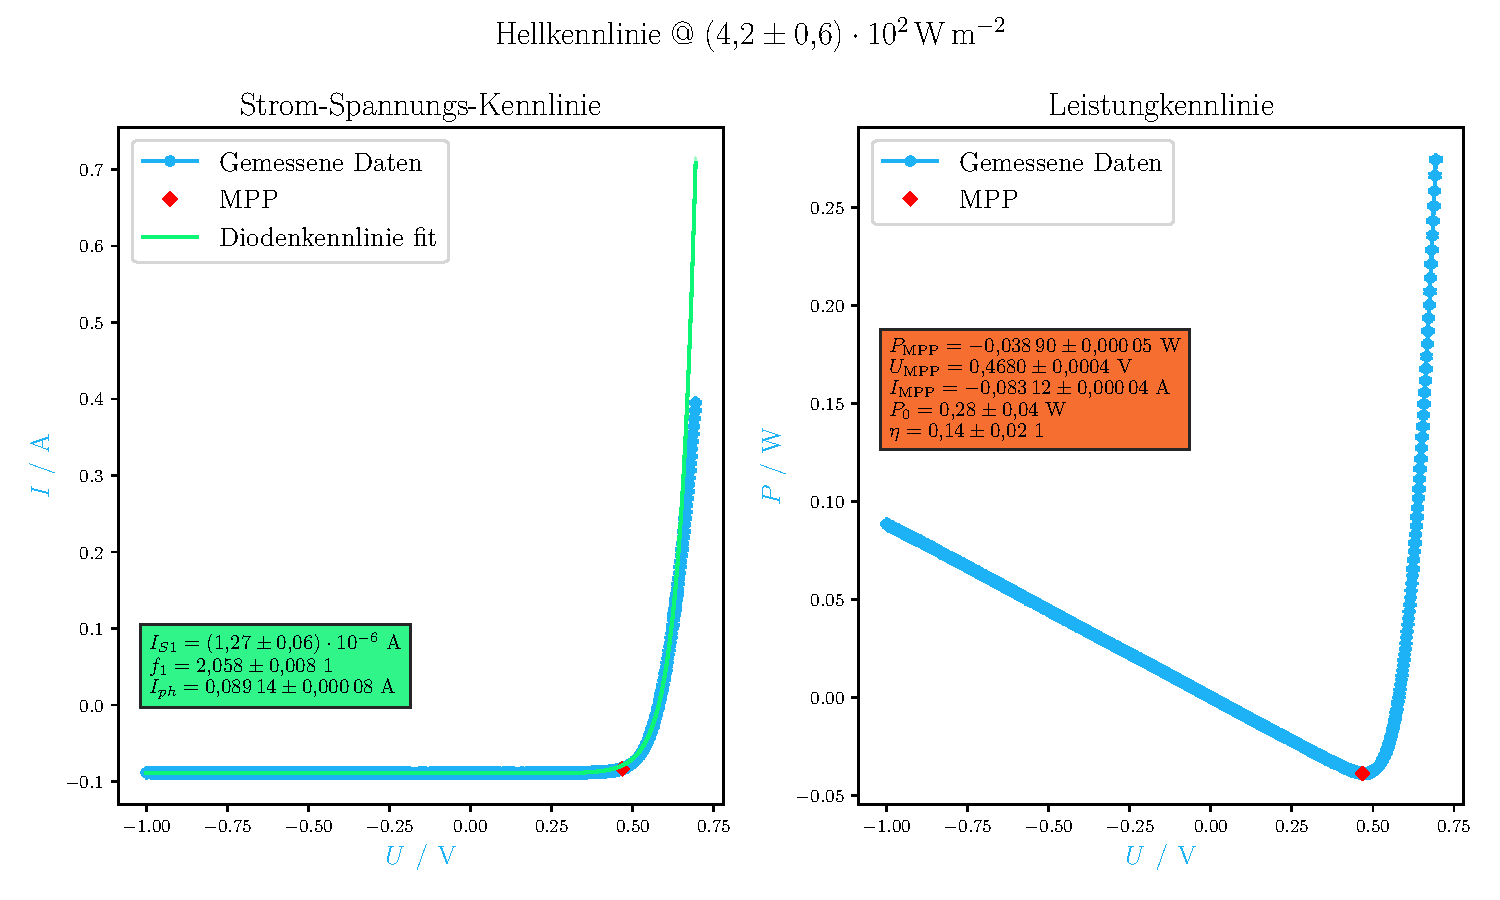
\includegraphics[width=0.95\textwidth]{figures/helllampe2.pdf}
	\caption[Kennlinie durch Halogen-Lampen 2.te Belichtung]{Untersuchung der
		Strom-Spannungs Kennlinie (links) und Leistungskennlinie (rechts) bei einer
		Bestrahlungsstärke der Solarzelle von \SI{420(60)}{\watt\per\meter\squared}
		mittels einer Halogenlampe. Folgende Größen wurden errechnet und, um Effizienz
		für dieser Konfiguration besser vergleichen zu können, auch angeführt: \\
		$P_\text{MPP} \dots$ Leistung am MPP                                   \\
		$I_\text{MPP} \dots$ Strom am MPP                                      \\
		$U_\text{MPP} \dots$ Spannung am MPP                                   \\
		$P_0 \dots$ Zugeführte Strahlungsfluss                                 \\
		$\eta \dots$ Wirkungsgrad
	}\label{fig:ausw_kennlinie_hell_lampe2}
\end{figure}

\begin{figure}[H]
	\centering
	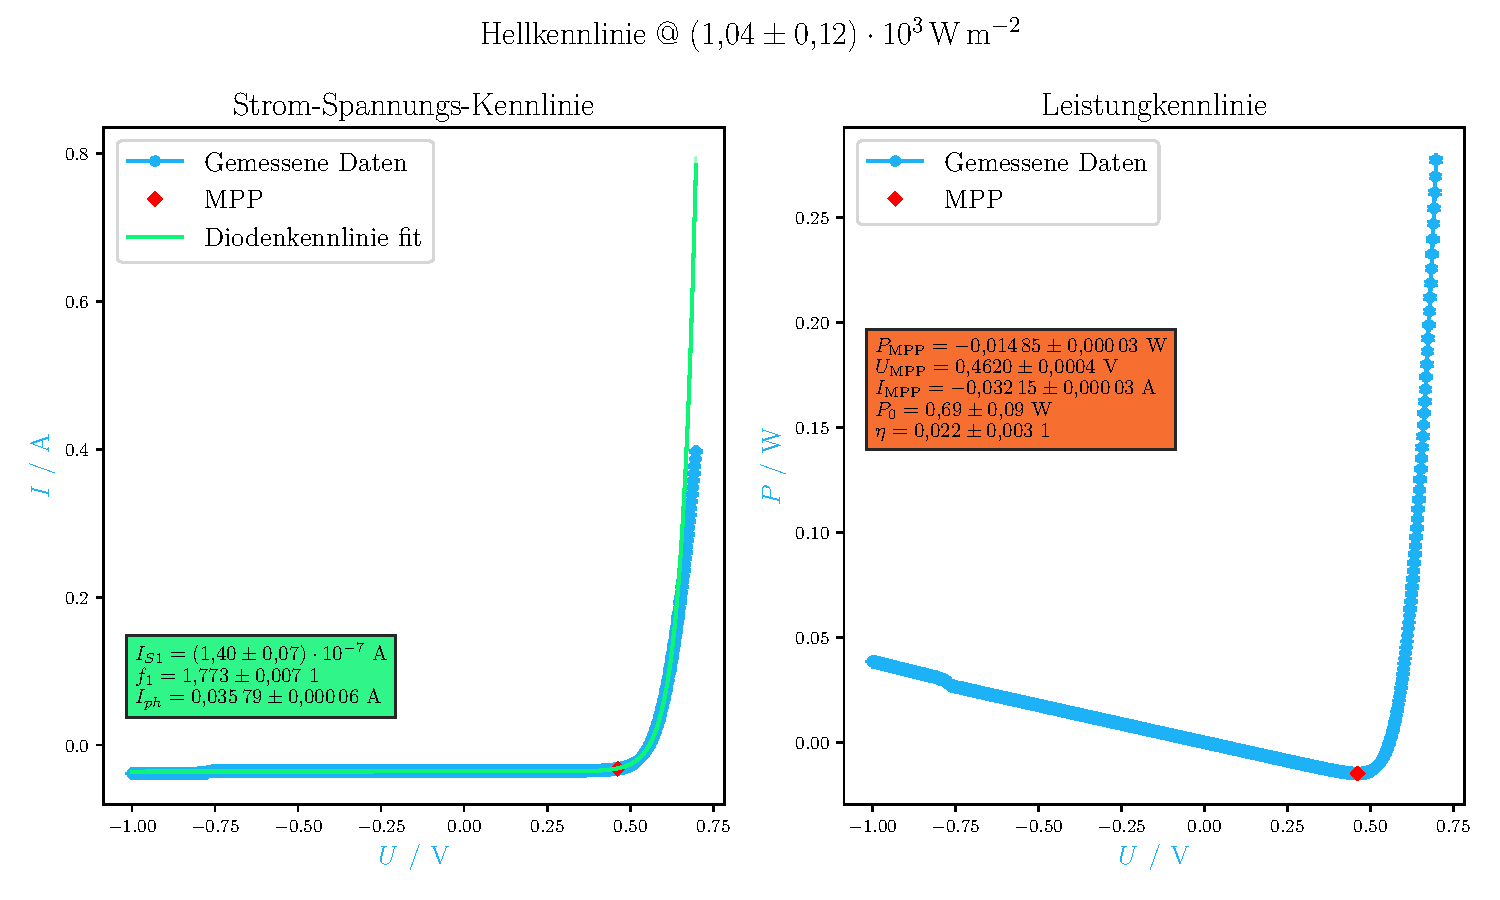
\includegraphics[width=0.95\textwidth]{figures/hellled.pdf}
	\caption[Kennlinie durch LED-Lampen Belichtung]{Untersuchung der Strom-Spannungs
		Kennlinie (links) und Leistungskennlinie (rechts) bei einer Bestrahlungsstärke
		der Solarzelle von \SI{1040(120)}{\watt\per\meter\squared} mittels einer
		bläulichen LED-Lampe. Folgende Größen wurden errechnet und, um Effizienz für
		dieser Konfiguration besser vergleichen zu können, auch angeführt: \\
		$P_\text{MPP} \dots$ Leistung am MPP                               \\
		$I_\text{MPP} \dots$ Strom am MPP                                  \\
		$U_\text{MPP} \dots$ Spannung am MPP                               \\
		$P_0 \dots$ Zugeführte Strahlungsfluss                             \\
		$\eta \dots$ Wirkungsgrad
	}\label{fig:ausw_kennlinie_hell_led}
\end{figure}

\section{Diskussion}\label{sec:diskussion}

\subsection{Wärmepumpe}

Beim Betrachten der Grafik in \autoref{fig:druckTemperaturVerlauf} wird klar
ersichtlich, dass es besser wäre die Flüssigkeit immer konstant umzurühren, da
sonst, immer wenn umgerührt wird, Spikes in den Temperatur und Druckverläufen
entstehen, die vermeiden werden sollten.

Nach dem Versuch beim Entfernen des Kübels wurde festgestellt, dass sich auf
der Kalten Seite Eis gebildet hat, wie in \autoref{fig:eis} sichtbar, welches
natürlich isolierende Auswirkungen hat und somit das Ergebnis verfälscht. Bei
einer erneuten Durchführung des Versuchs sollte daher die Flüssigkeit, nicht
nur wegen der Spikes sondern auch gegen die Eisbildung deutlich öfter umgerührt
werden.

\begin{figure}[H]
	\centering
	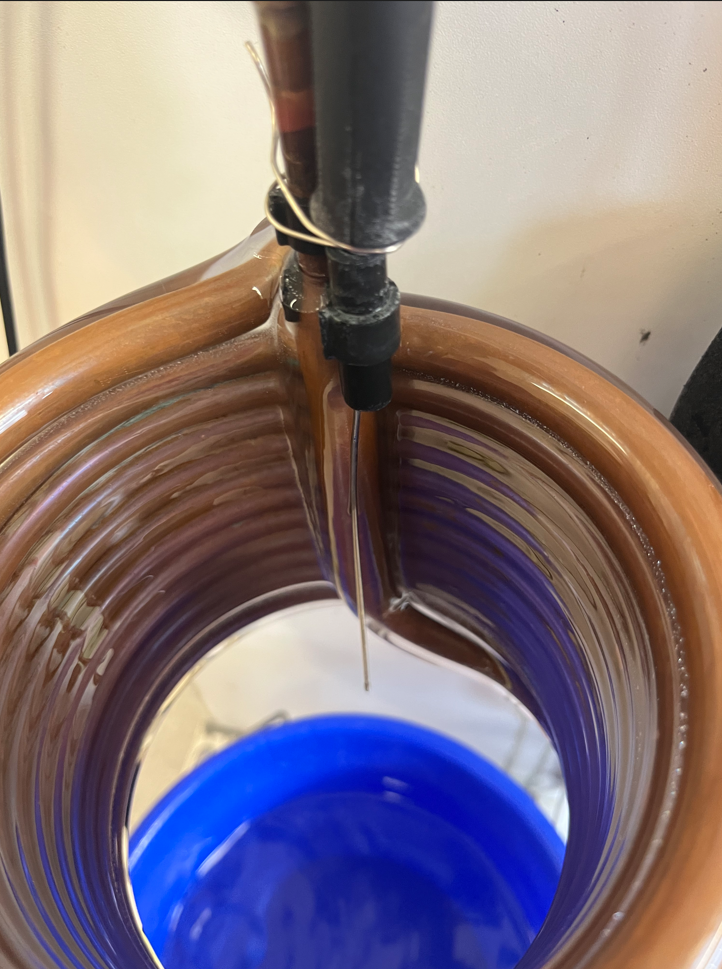
\includegraphics[width=0.5\textwidth]{figures/eis.PNG}
	\caption{Eisbildung
	}\label{fig:eis}
\end{figure}

\subsection{Kennlinien und Kenndaten von Solarzellen bei Bestrahlung}

Bei einer erneuten Durchführung wäre es wichtig, die Lampe einige Zeit auf die
Solarzelle scheinen zu lassen, damit sich eine konstante Betriebstemperatur
einstellen kann, bevor die Messung begonnen wird.

Die Solarzelle waren zur Lichtquelle verdreht, deshalb ist die effektive Fläche
mit dem Cosinus zur ganzen Fläche verbunden ($A' = A \cos(\theta)$). Der
dadurch entstandene prozentuelle Fehler beträgt somit
$100(1-\frac{A'}{A})=\SI{0.38}{\percent}$.

\subsubsection{Serienschaltung der beiden Solarzellen}

Ein Vergleich der Werte zeigt, dass die Serienschaltung eine höhere Spannung
bei einem niedrigeren Strom liefert, als die Parallelschaltung, wie es zu
erwarten war.

\subsubsection{Parallelschaltung der beiden Solarzellen}

Die Parallelschaltung bietet einen höheren Strom bei niedriger Spannung als die
Serienschaltung, wie bei Parallelschaltung üblich. Zudem ist die Leistung höher
als bei Serienschaltung, was der Ohmschen-Model widerspricht (eigentlich
sollten sie gleich sein). Da sich dieses aber nicht linear verhält ist dies
wahrscheinlich der Grund für die Diskrepanz zum Ohmschen-Model.

\subsubsection{Serienschaltung der beiden Solarzellen, wobei eine Solarzelle partiell abgeschattet wird}

Bei den teils bedeckten, in Serie geschalteten Solarzellen ist ein enormer
Abfall in der gewonnene Leistung vonstatten gegangen. Dies lässt sich erklären,
da die beschattete Fläche ein parasitärer Widerstand ist.

\subsection{Diodenparameter und Wirkungsgrad einer Solarzelle}

Bei der Dunkelkennlinie entsprechen die meisten Parameter(e.g.\ wie $I_{ph}$)
null was auch mit der Erwartung übereinstimmt.

Da die Bestrahlungsstärke mit dem Abstand zum Quadrat absinkt, ist der
gemessene Punkt nur ein Informations Punkt und nicht representative für die
gesamte Bestrahlungsstärke der Solarzelle. Deshalb wäre eine Technik, um die
Watt Messung wahrheitsgetreuer zu machen, sinnvoll. Dies kann zum Beispiel mit
einer Approximation der Abstrahlungsfläche durch Kugelfächen gemacht werden. Um
dies zu machen muss der Sensor ein Paar Punkte abfahren und dann ein
Flächenmittelwert, für die interessierte Fläche, erstellt werden.

Bei der bläulichen LED Lampe wird Energie schlechter von der Solarzellen
aufgenommen. Deshalb wird trotz der hohen Bestrahlungsstärke kaum etwas
konvertiert, da Solarzellen für das Sonnenabstrahlungsspektrum optimiert
werden.

\section{Zusammenfassung}\label{sec:zusammenfassung}

Hier werden nochmals alle Ergebnisse dieser Experimentenfolge aufgelistet.
Wobei die meisten zu erstellenden Diagramme Aufgrund der Länge der
\autoref{sec:auswertung} entnommen werden sollen.

\subsection{Wärmepumpe}
\begin{figure}[H]
	\centering
	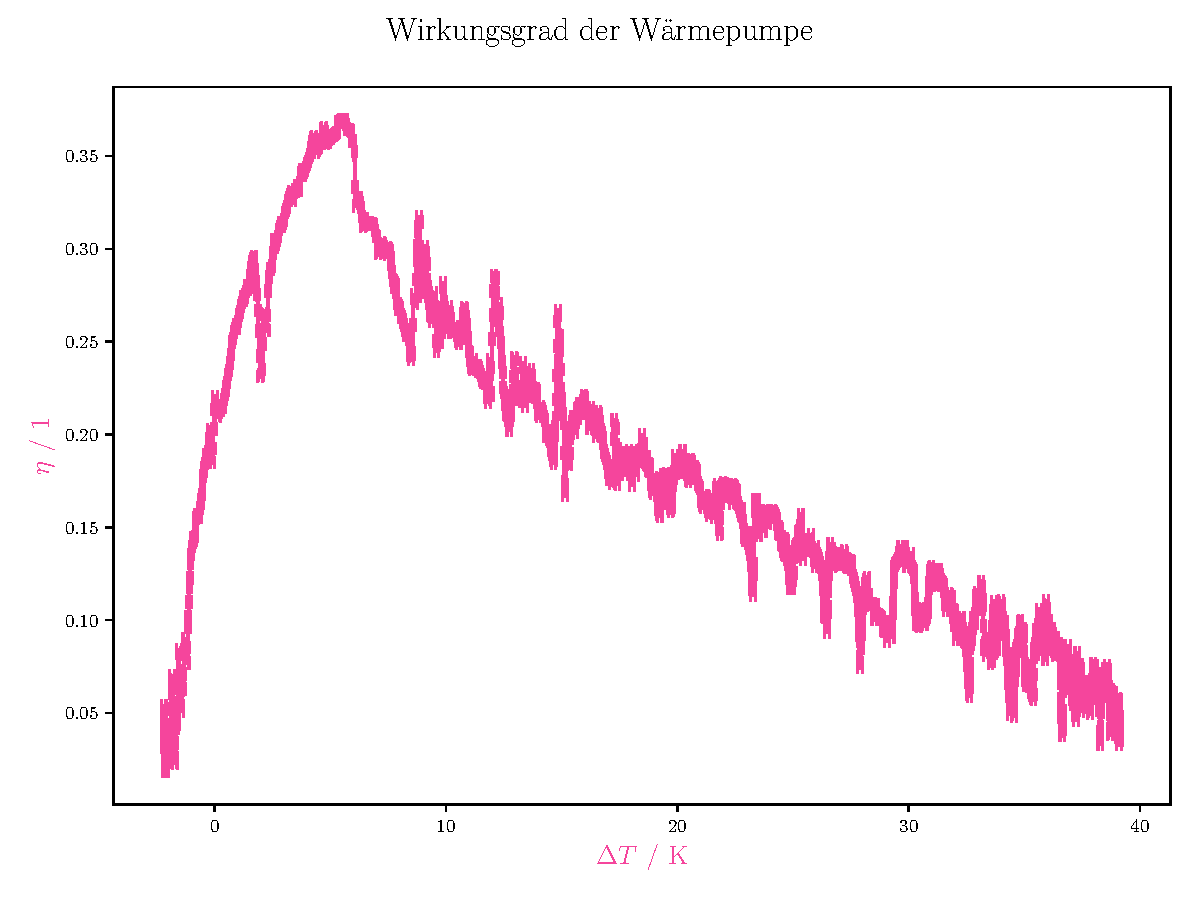
\includegraphics[width=0.95\textwidth]{figures/wirkungsgradVerlauf.pdf}
	\caption[Dynamischer Gütegradverlauf $\eta$ der Wärmepumpe]{Dynamischer Gütegradverlauf
		$\eta$ der Wärmepumpe. Der Gütegrad $\eta$ wird bezüglich der
		Temperaturdifferenz der zwei Reservoirs $\Delta T$ aufgetragen. Die, für diese
		Graphik errechnete, theoretisch maximale Leistungszahl $\epsilon_\text{max}$
		ist auch angeführt.
	}\label{fig:zusammenfassung}
\end{figure}

\subsection{Kennlinien und Kenndaten von Solarzellen bei Bestrahlung}

\begin{enumerate}
	\item $P_\text{MPP} = \SI{686(9)}{\milli\watt}$
	\item $U_\text{MPP} = \SI{10.120(18)}{\volt}$
	\item $I_\text{MPP} = \SI{67.8(7)}{\milli\ampere}$
	\item $U_L = \SI{12.03(3)}{\volt}$
	\item $I_k = \SI{76.6(8)}{\milli\ampere}$
	\item $FF = \SI{0.744(12)}{1}$
\end{enumerate}

\subsubsection{Serienschaltung der beiden Solarzellen}
\begin{enumerate}
	\item $P_\text{MPP} = \SI{891(11)}{\milli\watt}$
	\item $U_\text{MPP} = \SI{4.550(9)}{\volt}$
	\item $I_\text{MPP} = \SI{196(2)}{\milli\ampere}$
	\item $U_L = \SI{5.760(11)}{\volt}$
	\item $I_k = \SI{211(3)}{\milli\ampere}$
	\item $FF = \SI{0.734(12)}{1}$
\end{enumerate}

\subsubsection{Parallelschaltung der beiden Solarzellen}
\begin{enumerate}
	\item $P_\text{MPP} = \SI{43.7(6)}{\milli\watt}$
	\item $U_\text{MPP} = \SI{6.540(12)}{\volt}$
	\item $I_\text{MPP} = \SI{6.68(7)}{\milli\ampere}$
	\item $U_L = \SI{11.45(2)}{\volt}$
	\item $I_k = \SI{7.65(8)}{\milli\ampere}$
	\item $FF = \SI{0.499(9)}{1}$
\end{enumerate}

\subsubsection{Serienschaltung der beiden Solarzellen, wobei eine Solarzelle partiell abgeschattet wird}

\subsection{Diodenparameter und Wirkungsgrad einer Solarzelle}

Dunkelkennlinie:

\begin{enumerate}
	\item $f_1 = \SI{1.868(15)}{1}$
\end{enumerate}

Hellkennlinie Halogen Lampe $@\SI{250(30)}{\watt\per\meter\squared}$:

\begin{enumerate}
	\item $P_\text{MPP} = \SI{10.125(19)}{\milli\watt}$
	\item $U_\text{MPP} = \SI{0.4560(4)}{\volt}$
	\item $I_\text{MPP} = \SI{22.20(3)}{\milli\ampere}$
	\item $\eta = \SI{0.062(9)}{1}$
	\item $f_1 = \SI{1.668(5)}{1}$
\end{enumerate}

Hellkennlinie Halogen Lampe $@\SI{420(60)}{\watt\per\meter\squared}$:
\begin{enumerate}
	\item $P_\text{MPP} = \SI{38.90(5)}{\milli\watt}$
	\item $U_\text{MPP} = \SI{0.4680(4)}{\volt}$
	\item $I_\text{MPP} = \SI{83.12(4)}{\milli\ampere}$
	\item $\eta = \SI{0.14(2)}{1}$
	\item $f_1 = \SI{2.058(8)}{1}$
\end{enumerate}

Hellkennlinie bläuliche Led $@\SI{1040(120)}{\watt\per\meter\squared}$:
\begin{enumerate}
	\item $P_\text{MPP} = \SI{14.85(3)}{\milli\watt}$
	\item $U_\text{MPP} = \SI{0.4620(4)}{\volt}$
	\item $I_\text{MPP} = \SI{32.15(3)}{\milli\ampere}$
	\item $\eta = \SI{0.022(3)}{1}$
	\item $f_1 = \SI{1.773(7)}{1}$
\end{enumerate}

\newpage
\printbibliography
\listoffigures
\listoftables
\end{document}
